\documentclass[bachinf,zihtitle,german,final,hyperref,utf8]{res/zihpub}
\usepackage{enumitem}
\usepackage{graphicx}
\usepackage{subcaption}
\usepackage{hyperref}
\usepackage{listings}
\usepackage{wrapfig}
\usepackage[style=iso-alphabetic, maxcitenames=1, backend=biber]{biblatex}
\usepackage[nonumberlist, acronym, toc, section]{glossaries}
\setacronymstyle{long-short}
\renewcommand{\glsdisplayfirst}[4]{#1 #3}

\makeglossaries

\catcode`\ß=13
\defß{\ss}

\author{Jonas Schenke}
\title{Parallelisierung des Wellenfrontrekonstruktionsalgorithmus auf Multicore-Prozessoren}
\date{5. März 2018}

\matno{4055348}
\birthday{17. September 1995}
\placeofbirth{Burgstädt}
\gutachter{Prof. Thomas E. Cowan, PhD}
\betreuer{Dr. Michael Bussmann, Matthias Werner}

\copyrighterklaerung{
Die hier präsentierte Lösung basiert auf dem von Elena-Ruxandra Cojocaru implementierten Python Code, welcher wiederum auf Gundlage des MATLAB-Codes von Sébastien Bérujon erstellt wurde. Der Code der ursprünglichen Implementierung lässt sich auf dem GitHub-Repository \textit{Wavefront-Sensor} unter der General Public License finden\footnote{\url{https://github.com/ComputationalRadiationPhysics/Wavefront-Sensor/blob/master/LICENSE}} \cite{Coj17}.

Ebenso wurden, mit Erlaubniss der Ersteller, an der Beamline BM05 der \gls{ESRF} gemessene Daten zum Testen und Evaluieren verwendet. Dies waren die Datensätze \textit{Experiment 6}, welche am 24. September 2017 von Ruxandra Cojocaru, Sébastien Bérujon und Eric Ziegler aufgenommen wurde und die \textit{Lenses}-Datensätze, welche am zehnten April 2017 von Thomas Rothand, Raymond Barett, Sébastien Bérujon and Rafael Celeste erfasst wurden. 

Zur Implementierung des Wellenfrontrekonstruktionsalgorithmus wurden viele Open Source-Bibliotheken verwendet. Folgende Bibliotheken wurden hier besonders intensiv genutzt:
\begin{itemize}
	\item Cython (Apache Lizenz\footnote{\url{https://www.apache.org/licenses/LICENSE-2.0}})
	\item EdfFile.py (GPL Version 2\footnote{\label{gplv2}\url{https://www.gnu.org/licenses/gpl-2.0.html}})
	\item joblib (BSD\footnote{\label{bsd}\url{https://opensource.org/licenses/BSD-2-Clause}})
	\item matplotlib (matplotlib Lizenz\footnote{\url{https://matplotlib.org/users/license.html}})
	\item mpi4py (BSD\cref{bsd})
	\item numba (BSD\cref{bsd})
	\item NumPy (BSD 2.0\footnote{\label{bsd2}\url{https://opensource.org/licenses/BSD-3-Clause}})
	\item OpenCV (BSD\cref{bsd})
	\item Pillow (Standard PIL Lizenz\footnote{\url{http://www.pythonware.com/products/pil/license.htm}})
	\item Python (Python Software Foundation License\footnote{\url{https://www.python.org/download/releases/2.7/license/}})
	\item SciPy (SciPy Lizenz\footnote{\url{https://scipy.org/scipylib/license.html}})
\end{itemize}
}
\abstractde{\correctme{Ziel dieser Arbeit ist es, einen bereits in Python implementierten Wellenfrontrekonstruktionsalgorithmus zu beschleunigen. Dieser berechnet aus zwei Bildern eines zu untersuchenden Objekts pixelweise die die Fronten der elektromagnetischen Welle eines Röntgenlasers. Die Bilder werden dabei von zwei in einem festen zueinander Abstand stehenden, hochempfindlichen Röntgen-CCD-Sensoren aufgenommen. Die Kenntniss der Wellefront ist die Grundlage zur Phasenrekonstruktion bei Röntgenstreubildern aus denen die Struktur von Proben abgeleitet werden kann, die mit Hilfe des Röntgenlasers untersucht werden. Auf Basis von Performance-Analysen der Python-Implementierung sollen Optimierungen und Parallelisierungsmöglichkeiten für die kritischen Programmpfade ermittelt, implementiert und evaluiert werden. }}
\abstracten{\correctme{TODO}}
%Glosar
\newglossaryentry{uap}{name=\ensuremath{P_u},symbol=\ensuremath{P_u},description={Unterabtastperiode},first={Unterabtastperiode}}
\newglossaryentry{corrsize}{name=\ensuremath{R_{corr}},symbol=\ensuremath{R_{corr}},description={Korrelationsgröße bzw. Korrelationsauflösung},first={Korrelationsgröße}}
\newglossaryentry{resolution}{name=\ensuremath{R},symbol=\ensuremath{R},description={Auflösung},first={Auflösung}}
\newglossaryentry{rroi}{name=\ensuremath{R_{ROI}},symbol=\ensuremath{R_{ROI}},description={Auflösung der Region von Interesse},first={Auflösung der Region von Interesse}}
\newglossaryentry{N}{name=\ensuremath{N},symbol=\ensuremath{N},description={Anzahl der Bilder},first={Anzahl der Bilder}}
\newglossaryentry{N_Paare}{name=\ensuremath{N_{Paare}},symbol=\ensuremath{N_{Paare}},description={Anzahl der Bildpaare},first={Anzahl der Bildpaare}}
\newglossaryentry{gridResol}{name=\ensuremath{R_{grid}},symbol=\ensuremath{R_{grid}},description={Gitterauflösung},first={Gitterauflösung}}
\newglossaryentry{ncorr}{name=\ensuremath{N_{corr}},symbol=\ensuremath{N_{corr}},description={Anzahl der Korrekturversuche},first={Anzahl der Korrekturversuche}}
\newglossaryentry{nerr}{name=\ensuremath{N_{Err}},symbol=\ensuremath{N_{Err}},description={Anzahl der fehlerhaften Zuordnungen},first={Anzahl der fehlerhaften Zuordnungen}}
\newglossaryentry{rblock}{name=\ensuremath{R_{Block}},symbol=\ensuremath{R_{Block}},description={Auflösung der Blöcke},first={Auflösung der Blöcke}}
\newglossaryentry{npos}{name=\ensuremath{N_{Pos}},symbol=\ensuremath{N_{Pos}},description={Anzahl der Sensorpositionen},first={Anzahl der Sensorpositionen}}

%Abkürzungen
\newacronym{CCD}{CCD}{Charge-Coupled Device}
\newacronym{MPI}{MPI}{Message Passing Interface}
\newacronym{ROI}{ROI}{Region of Interest (Region von Interesse)}
\newacronym{FFT}{FFT}{Fast Fourier Transformation}
\newacronym{CPU}{CPU}{Central Processing Unit}
\newacronym{SSD}{SSD}{Solid-State Drive}
\newacronym{IO}{I/O}{Input/Output}
\newacronym{GHz}{GHz}{Gigahertz}
\newacronym{GB}{GB}{Gigabyte}
\newacronym{GiB}{GiB}{Gibibyte}
\newacronym{JIT}{JIT}{just-in-time}
\newacronym{GPGPU}{GPGPU}{General Purpose Computing on Graphics Processing Unit}
\newacronym{HZDR}{HZDR}{Helmholtz-Zentrum Dresden - Rossendorf e. V.}
\newacronym{ESRF}{ESRF}{European Synchrotron Radiation Facility}
\newacronym{EUCALL}{EUCALL}{European Cluster of Advanced Laser Light Sources}
\newacronym{UFDAC}{UFDAC}{Ultrafast Data Acquisition}
\newacronym{PUCCA}{PUCCA}{Pulse Characterisation and Control}
\addbibresource{res/Referenzen.bib}
\DefineBibliographyStrings{german}{
	andothers = {{\textit{et\,al\adddot}}},
}

\begin{document}
	\printglossary[title=Glossar, type=main]
	\printglossary[title=Abkürzungen,type=\acronymtype]
	\chapter{Einleitung}

\begin{correctmore}
	In dieser Arbeit wird ein bereits in Python implementierter Wellenfrontrekonstruktionsalgorithmus für Manycore-Prozessoren beschrieben.
	Die Wellenfront wird aus zwei Bildern ein und desselben Targets rekonstruiert, die von zwei CCD-Sensoren aus unterschiedlicher Entfernung aufgenommen werden. Aus den Unterschieden der Bilder lässt sich der Verlauf der Wellenfornten herleiten, welcher wiederum Aufschluss über die dreidimensionale Struktur des Targets gibt. 
	
	In seiner momentanen Implementierung benötigt der Algorithmus 25 Sekunden pro Bildpaar \textbf{nachprüfen}. Da die CCD-Sensoren mit bis zu 25 Bildern pro Sekunde erhebliche Datenmengen erzeugen, ist es wünschenswert diese Daten in-time zu verarbeiten, sodass eine Speicherung der Daten entfällt. 
	
	Soll-Kriterien, die hierbei an die parallele Lösung gestellt werden, sind zuallererst die Korrektheit der parallelen Implementierung und ein erheblicher Speedup \textbf{von wie viel?}, wobei eine echtzeitfähige Implementierung angestrebt wird.
\end{correctmore}	

\iffalse
- Anwendungsbeschriebung:
-> Wellenfrontrekonstruktionsalgorithmus liegt in Python implementiert vor
-> Rekonstruktion der Wellenfront aus Bildern 2er CCD Kameras in verschiedenem Abstand
- Motivation
-> momentaner Wellenfrontrekonstruktionsalgorithmus benötigt 25s/Frame
-> Kamera liefert 10 Frames/s
-> Daten müssen zwischengespeichert werden
- Einführen der Soll-Kriterien:
-> korrekte Rekonstruktion der Wellenfronten
-> deutliche Beschnleunigung der momentanen Implementierung (5x+)
\fi
	\chapter{Der Wellenfrontrekonstruktionsalgorithmus}

\section{Verwandte Arbeiten}

\subsection{Wellenfrontrekonstruktionsalgorithmus}

In strahlenphysikalischen Experimenten spielt die Ausrichtung optischer Bauteile und deren Qualität eine entscheidende Rolle. \citeauthor{GNS+11} beschrieben \citeyear{GNS+11} Methoden zur Messung dieser Fehler und zur Rekonstruktion der Wellenfront \cite{GNS+11}. Während der letzten zwei Jahrzehnte wurden hierzu verschiedene Techniken vorgestellt. \citeauthor{MZI+03} stellten \citeyear{MZI+03} ein Verfahren zur Ermittlung der Wellenfront unter Nutzung eines Hartmann-Sensors vor \cite{MZI+03}. \citeyear{WND+05} wurde von \citeauthor{WND+05} eine Methode zur Wellenfrontrekonstruktion mittels eines Gitterinferometers vorgestellt \cite{WND+05}. \citeauthor{APO+07} präsentierten \citeyear{APO+07} eine weitere Methode basierend auf der Verwendung einer Zufalls-Amplituden-Maske \cite{APO+07}. Diese umgeht das Problem der niedrigen räumlichen Auflösung eines Hartmann-Sensors und die aufwendige Kalibrierung der Optik eines Interferometers, indem mehrere Bilder in unterschiedlicher Entfernung vom zu untersuchenden Objekt gemacht werden. Dies bietet eine höhere Auflösung und die Möglichkeit, Ungenauigkeiten in der Optik algorithmisch zu korrigieren. Ein ähnlicher, robusterer Ansatz wurde \citeyear{Ber12} von \citeauthor{Ber12} unter Zuhilfenahme des X-Ray-Speckle-Traking-Algorithmus verfolgt \cite{Ber12} und \citeyear{Ber13} wurde von \citeauthor{Ber13} eine Methode mit zwei Sensoren vorgestellt, welche simultan Bilder des zu untersuchenden Objektes aufnehmen können und somit schneller sind \cite{Ber13}. Auf dieser Methode basiert der hier behandelte Wellenfrontrekonstruktionsalgorithmus. 

\subsection{Python-Optimierungen}

Es wurde von \citeauthor{Oli07} und \citeauthor{PGH11} aufgezeigt, dass die Programmiersprache Python aufgrund ihrer Simplizität und der Verfügbarkeit vieler Bibliotheken sich gut für wissenschaftliche Berechnungen eignet \cite{Oli07,PGH11}. Da Python als Skriptsprache nicht besonders schnell ist, wurde sich bereits ausgiebig mit dem Thema Beschleunigung von Python-Code beschäftigt. Die Lösungsansätze reichen von der Verwendung optimierter Bibliotheken über das Kompilieren kompletter Programme bis hin zur Vektorisierung und Parallelisierung des Codes. \citeyear{BR09} wurde von \citeauthor{BR09} sogar eine auf Loop-Unrolling und Bytecode-Optimierung basierende Methode vorgestellt \cite{BR09}. \citeauthor{Ill14} hat \citeyear{Ill14} einen Überblick über verschiedene Optimierungen gegeben und deren Effektivität anhand des freewake-Algorithmus aufgezeigt \cite{Ill14}.

\paragraph{Kompilieren}

\citeauthor{BBC+11} zeigten, dass mithilfe des Cython-Compilers und dessen Erweiterungen für Python unter bestimmten Szenarien die 1000-fache Geschwindigkeit erreicht werden kann. Dies ist möglich, indem der für Cython optimierte Python-Code nach C/C++ übersetzt und kompiliert wird \cite{BBC+11}. Ein weiterer, nennenswerter Python-zu-C++-Compiler ist der Shed-Skin-Compiler \cite{Mar09}. \citeauthor{LPS15} präsentierten \citeyear{LPS15} numba, einen Python Just-In-Time-Compiler \cite{LPS15}. Dieser unterstützt unter anderem auch Annotationen, mit denen sich einzelne Python-Funktionen unabhängig vom Rest des Programmes \gls{JIT} in nativen Code übersetzen lassen. 

\paragraph{Vektorisierung}

Wie man mittels Pythran und Boost.SIMD Python vektorisieren kann, wurde \citeyear{GFB14} von \citeauthor{GFB14} gezeigt \cite{GFB14}. Eine weitere Möglichkeit bietet die numpy-Bibliothek, welche eine einfache Anwendung von Rechenoperationen auf ganze Arrays zulässt. Die wichtigsten Funktionen der numpy-Bibliothek wurden von \citeauthor{VCV11} dargelegt. \citeauthor{Dai09} stellte \citeyear{Dai09} eine Bibliothek vor, die ähnliche Verfahren über mehrere Rechner verteilen kann \cite{Dai09}. \citeauthor{GBA13} stellten \citeyear{GBA13} einen Ansatz vor, mit dem sich auch OpenMP in Python nutzen lässt \cite{GBA13}. Eine MPI-1-Implementierung existiert ebenfalls und wurde \citeyear{DPS05} von \citeauthor{DPS05} vorgestellt und \citeyear{DPS+08} von \citeauthor{DPS+08} auf MPI-2 erweitert \cite{DPS05,DPS+08}. Die Verteilung der Daten auf verschiedene Rechenknoten kann erheblichen Einfluss auf die Leistung des Gesamtprogrammes haben. Um Python-Objekte zwischen Rechnern auszutauschen, müssen diese serialisiert werden, was mittels dem Python-internen Pickle/cPickle-Modul erreicht werden kann. Hierzu verglichen \citeauthor{DPK+11} die Pickle/cPickle-Methoden mit einer in C implementierten Buffer-Variante \cite{DPK+11}. Pickle/cPickle war dabei bis zu 30\% langsamer als die in C implementierten Buffer-Variante. 

\paragraph{Anwendungen}

Aufgrund der mannigfaltigen Möglichkeiten der Optimierung und der einfachen Nutzung, hält Python verstärkt Einzug auf Hochleistungsrechner. \citeauthor{KE14} präsentierten hierzu \citeyear{KE14}, wie Python-Code effizient auf der Intel\textregistered Xeon Phi\texttrademark Coprozessoren ausgeführt werden kann \cite{KE14}. Wie Python für Hochenergiephysik verwendet werden kann, zeigten \citeauthor{SKP+17} \cite{SKP+17}. Hierbei wurden die Bibliotheken numpy, HDF5 und mpi4py intensiv genutzt. Das von \citeauthor{HF17} vorgestellte nbodykit ist eine Ansammlung von Funktionen für Kosmologie-Simulationen, welche ebenfalls in Python entwickelt wurden und für den Gebrauch auf Hochleistungsrechnern optimiert wurde \cite{HF17}. Wie \citeyear{ERS+11} von \citeauthor{ERS+11} gezeigt wurde, kann Python auch auf Hochleistungsrechnern für die Simulation elektronischer Strukturen verwendet werden \cite{ERS+11}. Das Berechnen direkt numerischer Simulationen von Turbulenzverläufen kann laut \citeauthor{ML16} ebenfalls performant mit Python durchgeführt werden \cite{ML16}.

\section{Einführung}

\subsection{Versuchsaufbau}

\begin{figure}[h!]
	\begin{center}
		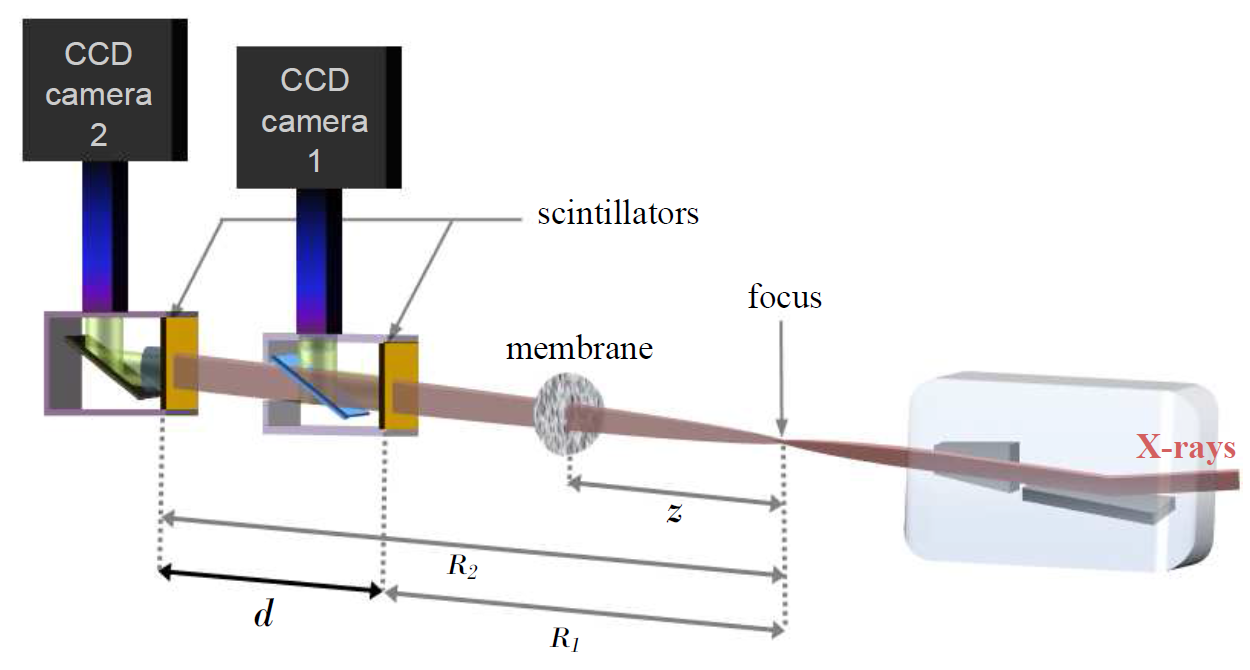
\includegraphics[width=0.9\textwidth]{img/Versuchsaufbau}
		\caption[Versuchsaufbau]{Versuchsaufbau \shortcite{Ber15}{891}}
		\label{fig:versuch}
	\end{center}
\end{figure}

Ein allgemeiner Versuchsaufbau in der Strahlenphysik besteht aus einer Röntgenstrahlenquelle, einem zu untersuchenden Objekt, welches im Fokus der Röntgenstrahlen platziert ist, und einem Aufnahmeaufbau, wie es von \citeauthor{Ber13} beschrieben wurde \shortcite{Ber13}{31 ff.}. Mittels der Belichtung des zu untersuchenden Objekts können anschließend physikalische Informationen über dieses herausgefunden werden.

\citeauthor{Ber13} zeigte ebenfalls, dass die Bestimmung der geometrischen Struktur eines zu untersuchenden Objekts mittels eines solchen Versuchsaufbaus realisiert werden kann \shortcite{Ber13}{105 ff.}. Der Aufnahmeaufbau, laut \citeauthor{Ber15}, besteht in diesem konkreten Fall aus einer Fleckenmembran und zwei hochempfindlichen Röntgen-\gls{CCD}-Sensoren, die zwei Bilder des zu untersuchenden Objekts zeitgleich aus unterschiedlicher Entfernung durch die Fleckenmebran aufnehmen \shortcite{Ber15}{887}. Ein solcher Versuchsaufbau wird in der Abbildung \ref{fig:versuch} dargestellt, welche aus der Veröffentlichung \cite{Ber15} von \citeauthor{Ber15} entnommen wurde.

Die Röntgenstrahlen werden zuerst am zu untersuchenden Objekt absorbiert und gebrochen und treffen anschließend auf die Membran, wodurch das Röntgenstrahlbündel hinter dieser Membran ein Fleckenmuster aufweist. Dieses Bündel trifft zuerst auf den Szintillator des ersten \gls{CCD}-Sensors, welcher die Röntgenstrahlen für die \gls{CCD}-Sensoren sichtbar macht. Der sichtbare Teil dieses Bildes wird zum erstem \gls{CCD}-Sensor reflektiert und dort aufgenommen. Der Röntgen-Teil wird zum Szintillator des zweiten \gls{CCD}-Sensors gebrochen, wo dieser in sichtbares Licht gewandelt wird, das mittels einer Optik zum zweiten \gls{CCD}-Sensor reflektiert und dort aufgenommen wird. \shortcite{Ber15}{886 ff.}

Aus der Verschiebung der Flecken lässt sich die Phase, und somit die Wellenfront des Lichtes, rekonstruieren, wozu der Wellenfrontrekonstruktionsalgorithmus verwendet wird. Gemäß \citeauthor{Ber13} besteht dieser aus zwei Teilen, welche im Folgenden genauer beschrieben werden sollen: einer Kalibrierung der \gls{CCD}-Sensoren und der Hauptverarbeitungsroutine der Bilder \shortcite{Ber13}{194}. Der Algorithmus soll online (zeitgleich zum Experiment) ausgeführt werden. Die \gls{CCD}-Sensoren haben eine Auflösung von 2048 mal 2048 Pixeln mit einer Farbtiefe von 16 Bit (Graustufen) und liefern bis zu 10 Bilder pro Sekunde.

\subsection{Kalibrierung der CCD-Sensoren}

\begin{figure}[h!]
	\centering
	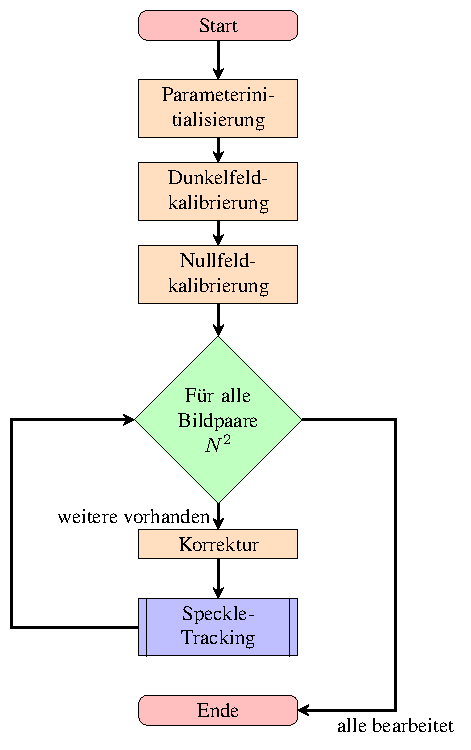
\includegraphics[width=0.45\textwidth]{pdf/graph_init}
	\caption[Kalibrierung]{Programmablaufplan der Kalibrierung (nach \shortcite{Ber13}{85 ff., S. 194} und \cite{Coj17}; angefertigt gemäß DIN 66001 bzw. ISO 5807)}
	\label{fig:graph_kalibrierung}
\end{figure}

Während der Kalibrierung findet, gemäß \citeauthor{Ber13}, zuerst eine Parameterinitialisierung statt, nach welcher der Kamerafehler der \gls{CCD}-Sensoren in drei Phasen bestimmt wird \shortcite{Ber13}{76 ff., S. 194}. Dazu wird, wie in Abbildung \ref{fig:graph_kalibrierung} gezeigt, zuerst der Median aus einer festen Anzahl dunkler Bilder aufgenommen, was auch als Dunkelfeldkalibrierung bezeichnet wird. Anschließend findet eine Nullfeldkalibrierung statt, in welcher bei ungestörter Wellenfront der Verstärkungsfaktor der einzelnen Pixel ermittelt wird. Zum Schluss findet eine Erkennung von Streueffekten im Detektor statt. Um letzteres zu erreichen, werden für jeden \gls{CCD}-Sensor \glssymbol{npos}$^2$ Bilder unter Bewegung der \gls{CCD}-Sensoren aufgenommen, wobei \glssymbol{npos} hier gleich der Anzahl der Verschiebungen in X- und Y-Richtung ist. Dadurch lässt sich aus den vertikalen und horizontalen Gradienten benachbarter Motorpositionen die jeweilige Streuung der Sensoren mittels des Speckle-Trackings bestimmen. Aus diesen \glssymbol{npos} Positionen ergibt sich somit, dass die \gls{N} gleich $\glssymbol{npos} \cdot \left(\glssymbol{npos} - 1\right) \cdot 2 \cdot 2$ ist, da jeweils horizontal und vertikal $\glssymbol{npos} \cdot \left(\glssymbol{npos} - 1\right)$ Bildpaarkombinationen existieren, welche in beide Richtungen miteinander verrechnet werden müssen. Da die Kalibrierung lediglich am Anfang des Experiments einmal durchgeführt werden muss, wird diese im weiteren Verlauf der Arbeit vernachlässigt. 

\paragraph{Speckle-Tracking}
\label{sec:speckle-tracking}

\begin{center}
	\begin{figure}[h!]
		\centering
		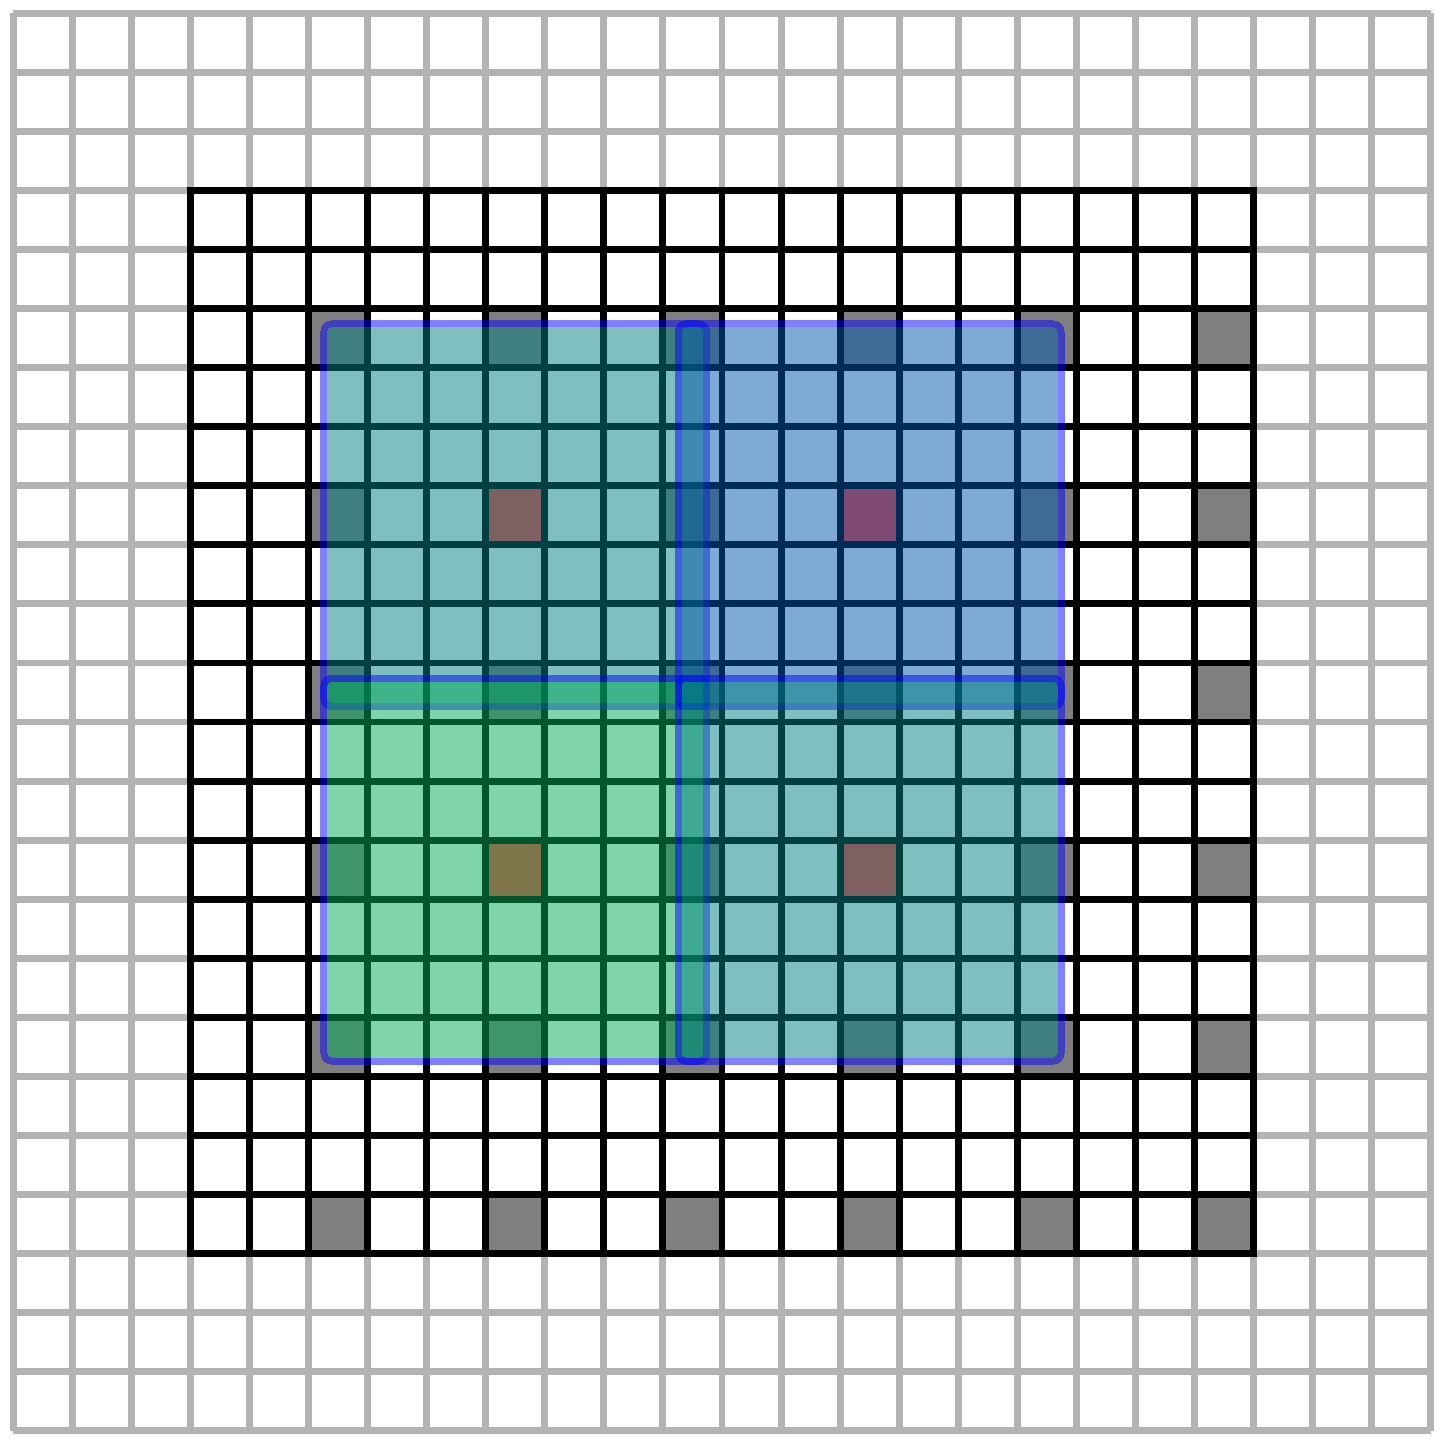
\includegraphics[width=0.5\textwidth]{pdf/template_matching}
		\quad
		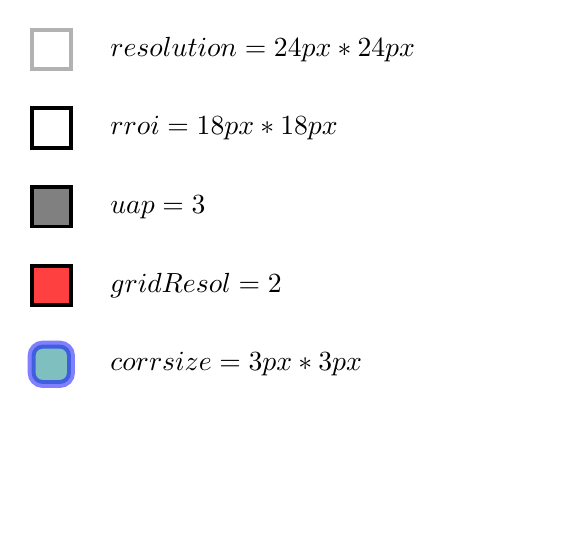
\begin{tikzpicture}[node distance=1cm]
		\node[rectangle, draw=black!30, minimum width=0.5cm, minimum height=0.5cm, line width=0.5mm](pixel) at (0,0){};
		\node[rectangle, draw, minimum width=0.5cm, minimum height=0.5cm, line width=0.5mm, below of=pixel](node){};
		\node[rectangle, draw, fill=black!50, minimum width=0.5cm, minimum height=0.5cm, line width=0.5mm, below of=node](sample){};
		\node[rectangle, draw, fill=red!75, minimum width=0.5cm, minimum height=0.5cm, line width=0.5mm, below of=sample](grid){};
		\node[rectangle, rounded corners, draw=blue, fill={rgb:blue,1;green,1}, opacity=0.5, minimum width=0.5cm, minimum height=0.5cm, line width=1mm, below of=grid](corr){};
		
		\node[text width=5.5cm, xshift=2.5cm, right of=pixel](pixel_desc){$\glssymbol{resolution} = 24 px * 24 px$};
		\node[text width=5.5cm, below of=pixel_desc](node_desc){$\gls{rroi} = 18 px * 18 px$};
		\node[text width=5.5cm, below of=node_desc](sample_desc){$\gls{uap} = 3$};
		\node[text width=5.5cm, below of=sample_desc](grid_desc){$\gls{gridResol} = 2$};
		\node[text width=5.5cm, below of=grid_desc](corr_desc){$\gls{corrsize} = 3 px * 3 px$};
		
		\node[]() at (0, -6cm){};
		\end{tikzpicture}
		\caption{Übersicht der Template-Matching-Parameter im zweiten Durchlauf}
		\label{fig:tm_param}
	\end{figure}
\end{center}

Ziel des Speckle-Trackings ist es, die Flecken (englisch: speckle) zwischen den \gls{CCD}-Sensoren zu verfolgen, welche von der Fleckenmembran geworfen werden. Der von \citeauthor{Ber13} beschriebene Speckle-Tracking-Algorithmus (dargestellt in Abbildung \ref{fig:graph_speckle}) ermittelt zuerst die starre Verschiebung der beiden Sensoren zueinander \shortcite{Ber13}{76 ff., S. 194}. Dies kann mittels festgelegter Werte, Korrelation oder Kreuzkorrelation geschehen. Anschließend werden die Bilder der Sensoren in 35 mal 35 Pixel bzw. 10 mal 10 Pixel große Teilbilder aufgeteilt, damit ein grober Gradient in einem ersten Durchlauf (gezeigt in Abbildung \ref{fig:graph_first}) bestimmt werden kann. Diese Teilbilder liegen hierbei alle in der \gls{ROI}, welche die möglicherweise fehlerbehafteten Bildränder abschneidet. Die Verschiebung der Teilbilder zwischen den beiden Bildern der Sensoren wird mithilfe des von \citeauthor{Lew94} beschriebenen Template-Matching-Prozesses ermittelt \cite{Lew94}. Dieser sucht die Teilbilder des ersten Sensors mit denen des zweiten Sensors, wobei eine Übereinstimmungsmatrix entsteht. Anhand der Positionen der Maxima kann nun die Verschiebung abgelesen werden. Dieser Prozess kann laut \citeauthor{Lew94} durch die Kreuzkorrelation der beiden Teilbilder im Frequenzraum realisiert werden um die Komplexität des Algorithmus zu senken \cite{Lew94}. Damit endet der erste Durchlauf. Im weiteren Verlauf werden zuerst stark abweichende Werte herausgefiltert und anschließend werden Ebenen an die horizontalen und vertikalen Verschiebungsmatrizen angelegt. Diese sind zur Interpolation nötig, da die Verschiebungsmatrizen lediglich einen Pixel pro Teilbild beinhalten. Sobald die Ebene auf die volle Auflösung des Bildes interpoliert wurde, wird der zweite Durchlauf (gezeigt in Abbildung \ref{fig:graph_second}) durchgeführt. Im diesem Durchlauf werden wieder beide Bilder in Teilbilder unterteilt, diesmal können sich die Teilbilder jedoch überlappen. Die konkrete Anzahl der Teilbilder hängt, gemäß des von \citeauthor{Coj17} entwickelten Codes, von drei Variablen ab \cite{Coj17}: der \gls{uap}, der \gls{corrsize} und der \gls{gridResol}. Mittels der Unterabtastperiode lassen sich, wie in Abbildung \ref{fig:tm_param} veranschaulicht, jeweils \gls{uap} Pixel überspringen, wodurch die effektive \gls{rroi} des Bildes auf \glsdesc{resolution} $\lfloor\glssymbol{rroi}/\gls{uap}^2\rfloor$ reduziert wird. Die \glsfirst{corrsize} \gls{corrsize} gibt die Größe der Teilbilder an. Die \glsfirst{gridResol} bestimmt die Größe des Resultats, indem jeweils ein Teilbild um jeden \gls{gridResol}-ten Punkt im bereits durch Unterabtastung verkleinerten Bild genutzt wird. Die Verschiebung der so berechneten Teilbilder wird dann mittels des Template-Matching-Prozesses bestimmt und auf Subpixel-Genauigkeit interpoliert. Teilbilder, die im zweiten Durchlauf nicht korrekt zugeordnet werden konnten, werden gesammelt und unter Verwendung von anderen Korrelationsgrößen erneut verarbeitet. Sollten diese Korrelationen ebenfalls fehlschlagen, werden die Ergebnisse der fehlerhaften Teilbilder interpoliert. 

\begin{figure}[h!]
	\centering
	\begin{subfigure}[b]{0.3\textwidth}
		\centering
		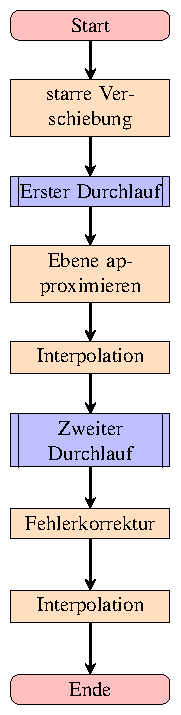
\includegraphics[width=0.5\textwidth]{pdf/graph_speckle}
		\caption[Speckle-Tracking]{Speckle-Tracking-Algorithmus (nach \shortcite{Ber13}{85 ff., S. 194} und \cite{Coj17})}
		\label{fig:graph_speckle}
	\end{subfigure}
	\hfill
	\begin{subfigure}[b]{0.3\textwidth}
		\centering
		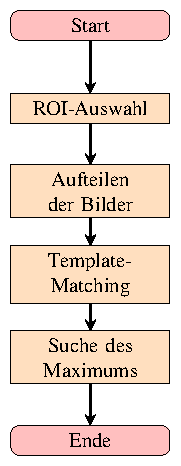
\includegraphics[width=0.6\textwidth]{pdf/graph_first_pass}
		\caption[Erster Durchlauf]{Erster Durchlauf (nach \cite{Ber12} und \cite{Coj17})}
		\label{fig:graph_first}
	\end{subfigure}
	\hfill
	\begin{subfigure}[b]{0.3\textwidth}
		\centering
		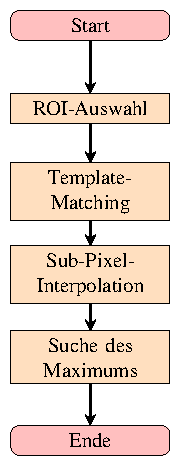
\includegraphics[width=0.6\textwidth]{pdf/graph_second_pass}
		\caption[Zweiter Durchlauf]{Zweiter Durchlauf (nach \shortcite{Ber13}{194}, \cite{Ber12} und \cite{Kov04})}
		\label{fig:graph_second}
	\end{subfigure}
	\caption[Algorithmen]{Programmablaufpläne der Speckle-Tracking-Subroutinen (angefertigt gemäß DIN 66001 bzw. ISO 5807)}
\end{figure}

\subsection{Verarbeitungsroutine der Bilder}

Die von \citeauthor{Ber15} beschriebene Hauptverarbeitungsroutine (siehe Abbildung \ref{fig:graph_hauptroutine}) ähnelt stark der Kalibrierung: Auch hier findet zuerst eine Parameterinitialisierung statt, welche von der Hauptschleife gefolgt wird \shortcite{Ber15}{891}. Diese verarbeitet hier, im Gegensatz zur Kalibrierung, nur jedes Bildpaar (Beispiel: Abbildung \ref{fig:eingabebilder}). Innerhalb der Hauptschleife gibt es auch hier die Korrektur der Sensorfehler und das anschließende Speckle-Tracking, dessen Ergebnisse in Abbildung \ref{fig:gradienten} gezeigt sind. Die Korrektur bezieht hierbei die von der Kalibrierung berechneten Ergebnisse, insbesondere die ermittelten Streueffekte der Sensoren. Anders als bei der Kalibrierung werden hierbei jedoch in der Hauptschleife die beiden Gradientenmatrizen mittels des von \citeauthor{FC88} entwickelten Algorithmus zu einer Phasenmatrix integriert (gezeigt in Abbildung \ref{fig:graph_fc}), was effizient im Frequenzraum möglich ist \cite{FC88}. Die zu in den Abbildung \ref{fig:eingabebilder} gezeigten Eingabebildern zugehörige Phasenmatrix ist in Abbildung \ref{fig:ausgabebild} dargestellt. Die in Abbildung \ref{fig:eingabebilder}, \ref{fig:gradienten} und \ref{fig:ausgabebild} gezeigten Daten sind Teil des \textit{Lenses Set 1}-Datensatzes, welcher am zehnten April 2017 von Thomas Roth, Raymond Barett, Sébastion Bérujon und Rafael Celeste an der Beamline BM05 der \gls{ESRF} aufgenommen wurde \cite{RBB+17}. 

\begin{figure}[h!]
	\centering
	\begin{subfigure}[b]{0.45\textwidth}
		\centering
		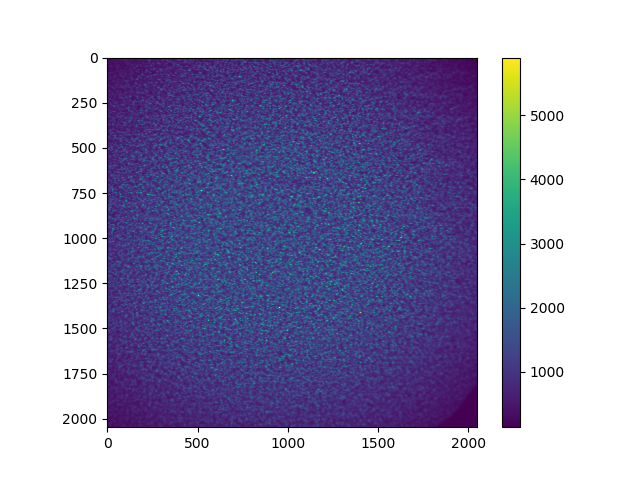
\includegraphics[width=\textwidth]{img/ref_start0001_1-10}
		\caption[Erster Sensor]{Eingabebild des ersten Sensors}
		\label{fig:eingabe_sensor1}
	\end{subfigure}
	\begin{subfigure}[b]{0.45\textwidth}
		\centering
		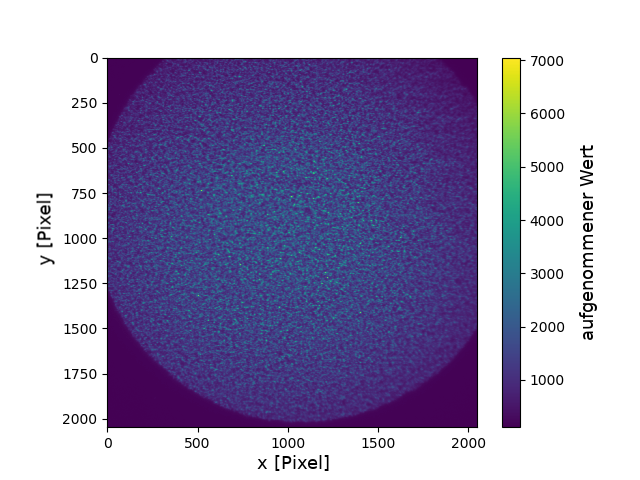
\includegraphics[width=\textwidth]{img/E10001}
		\caption[Zweiter Sensor]{Eingabebild des zweiten Sensors}
		\label{fig:eingabe_sensor2}
	\end{subfigure}
	\caption[Eingabe]{Eingabebilder (aufgenommen von Roth, Barett, Bérujon und Celeste an der Beamline BM05 \cite{RBB+17})}
	\label{fig:eingabebilder}
\end{figure}

\begin{figure}[h!]
	\centering
	\begin{subfigure}[b]{0.45\textwidth}
		\centering
		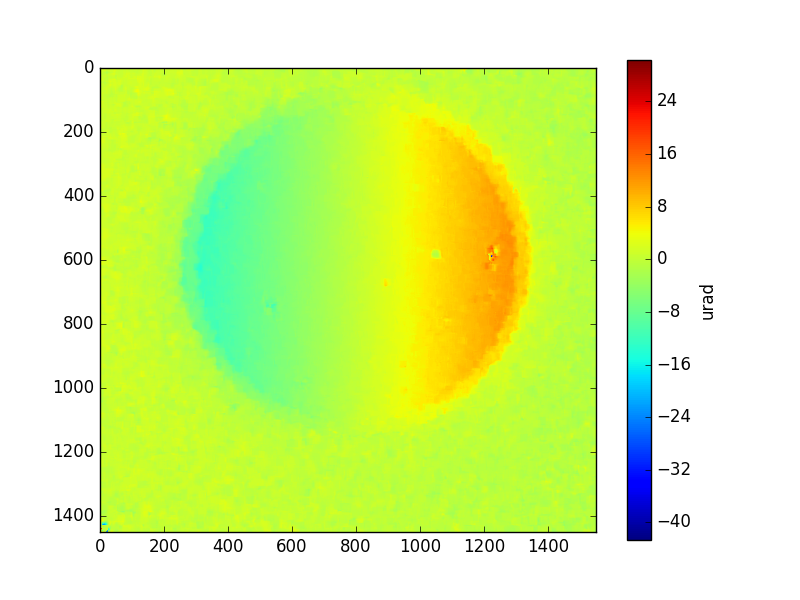
\includegraphics[width=\textwidth]{img/SpeckDisH_E10001_edf_ref_start0001_1-10_edf}
		\caption[Horizontaler Gradient]{Horizontaler Gradient}
		\label{fig:hor_grad}
	\end{subfigure}
	\begin{subfigure}[b]{0.45\textwidth}
		\centering
		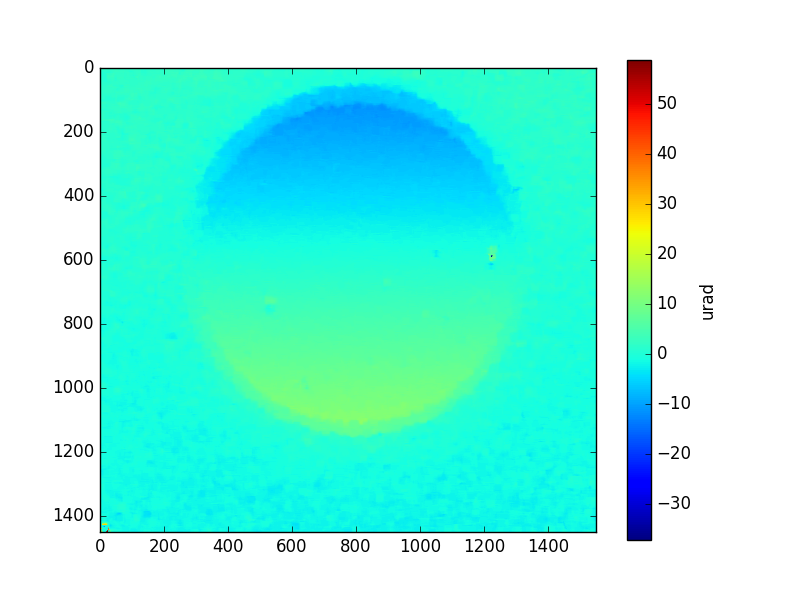
\includegraphics[width=\textwidth]{img/SpeckDisV_E10001_edf_ref_start0001_1-10_edf}
		\caption[Vertikaler Gradient]{Vertikaler Gradient}
		\label{fig:vert_grad}
	\end{subfigure}
	\caption[Gradient]{Gradientenbilder (Ausgabe des Speckle-Tracking, erstellt aus von Roth, Barett, Bérujon und Celeste an der Beamline BM05 aufgenommenen Daten \cite{RBB+17})}
	\label{fig:gradienten}
\end{figure}

\begin{figure}[h!]
	\centering
	\begin{subfigure}[b]{0.45\textwidth}
		\centering
		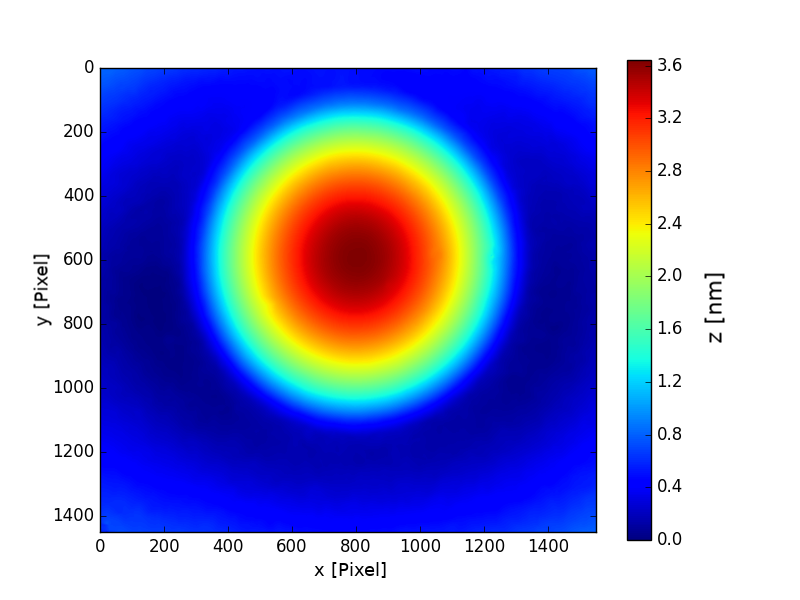
\includegraphics[width=\textwidth]{img/2D_E10001_edf_ref_start0001_1-10_edf}
		\caption[2D Ausgabe]{2D Repräsentation}
		\label{fig:ausgabe_2d}
	\end{subfigure}
	\begin{subfigure}[b]{0.45\textwidth}
		\centering
		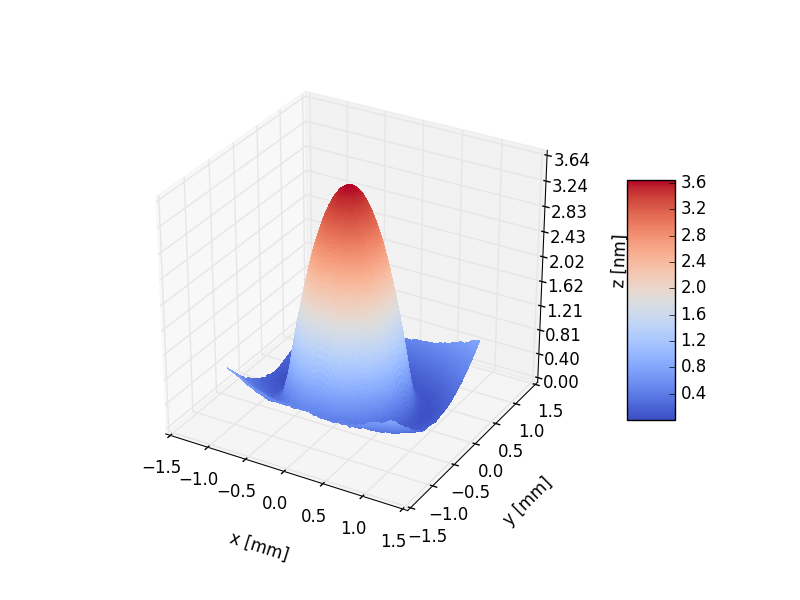
\includegraphics[width=\textwidth]{img/3D_E10001_edf_ref_start0001_1-10_edf}
		\caption[3D Ausgabe]{3D Repräsentation}
		\label{fig:ausgabe_3d}
	\end{subfigure}
	\caption[Ausgabe]{Ausgabe des Algorithmus (Phasenmatrix, erstellt aus von Roth, Barett, Bérujon und Celeste an der Beamline BM05 aufgenommenen Daten \cite{RBB+17})}
	\label{fig:ausgabebild}
\end{figure}

\begin{figure}[h!]
	\begin{subfigure}[b]{0.45\textwidth}
		\centering
		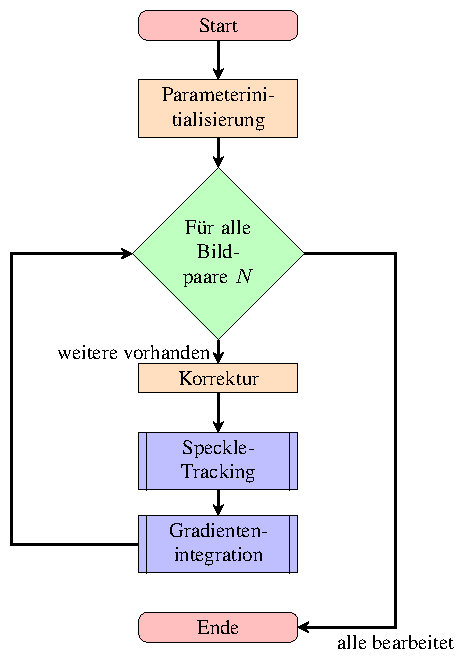
\includegraphics[width=\textwidth]{pdf/graph_main}
		\caption[Hauptroutine]{Hauptroutine (nach \shortcite{Ber13}{194} und \cite{Coj17})}
		\label{fig:graph_hauptroutine}
	\end{subfigure}
	\hfill
	\begin{subfigure}[b]{0.45\textwidth}
		\centering
		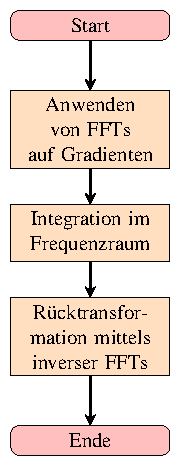
\includegraphics[width=0.4\textwidth]{pdf/graph_fc}
		\caption[Frankot-Chellappa]{Integration der Gradienten gemäß \cite{FC88} und \cite{Kov04}}
		\label{fig:graph_fc}
	\end{subfigure}
	\caption[Algorithmen]{Programmablaufpläne der Hauptroutine (angefertigt gemäß DIN 66001 bzw. ISO 5807)}
\end{figure}

\section{Die vorgegebene Python-Implementierung}

Der bestehende Python-Code wurde von Elena-Ruxandra Cojocaru auf Grundlage des von Sébastion Bérujon erstellten MATLAB-Codes entwickelt und ist auf dem GitHub-Repository \textit{Wavefront-Sensor} verfügbar \cite{Coj17}. Aufgrund der Abhängigkeit der Bibliothekt \textit{EdfFile} zum Auslesen der Bilddaten, wurde der Code in Python 2.7 geschrieben. Der Code ist in vier Dateien aufgeteilt. Die Datei \textit{norm\_xcorr.py} nutzt die Schnittstelle zu der in OpenCV implementierten Template-Matching-Funktion \cite{SA17}. Alle Helferfunktionen, insbesondere die des Speckle-Trackings und die der Integration der Gradienten, befinden sich in der Datei \textit{func.py}. Der Code der Kalibrierung befindet sich in der \textit{detectorDistortion.py} Datei und der der Hauptroutine befindet sich in der Datei \textit{wavefront.py}. 

\subsection{Überblick}

\begin{sloppypar}
	Die Datei \textit{norm\_xcorr.py} enthält alle Funktionen, die für das Template-Matching benötigt werden. Darunter ist die Funktion \texttt{norm\_xcorr()}, welche lediglich als Schnittstelle für die Template-Matching Funktion aus OpenCV dient. Sie nimmt als Argumente ein Template, ein Suchfeld und optional den Namen des gewünschten Algorithmus entgegen und gibt die Übereinstimmungsmarix, die Position und den Wert des Maximums und des Minimums zurück. Die zweite Funktion in dieser Datei ist die \texttt{nxcorr\_disp()}-Funktion, welche die Übereinstimmungsmatrix an relevanten Stellen, wo die Übereinstimmung am höchsten ist, auf ein Subpixel-Level verfeinert. Dazu nimmt diese Funktion das Ergebnis der \texttt{norm\_xcorr()}-Funktion entgegen und gibt die Position sowie den Wert des neuen Maximums und das Signal-Rausch-Verhältnis zurück. \cite{Coj17}
\end{sloppypar}

Die \textit{func.py} enthält die meisten Helferfunktionen. Dazu gehören unter anderem Funktionen zur \gls{ROI}"=Auswahl und verschiedene Filterfunktionen. Des Weiteren befinden sich in dieser Datei auch die Funktionen \texttt{computerCorrField()} und \texttt{correction()}.\texttt{ computerCorrField()} berechnet aus Bildern an einem vorgegebenen Pfad entweder das mediangefilterte Bild für die Dunkelfeld-Kalibrierung oder das durchschnittsgefilterte Bild für Nullfeld-Kalibrierung. Mithilfe der \texttt{correction()}-Funktion können nun diese berechneten Korrekturbilder auf Eingabebilder mittels Subtraktion für die Dunkelfeld-Kalibrierung oder mittels Division für die Nullfeld-Kalibrierung angewendet werden. Zwei weitere wichtige Funktionen sind \texttt{firstPass()} und \texttt{cpCorr()}, welche den ersten (\texttt{firstPass()}) und zweiten Durchlauf (\texttt{cpCorr()}) implementieren. Diese sind damit Teil des Speckle-Trackings-Algorithmus, welcher in der \texttt{crossSpot4()}-Funktion implementiert ist. Die letzte wichtige Funktion im \texttt{func.py}-Skript ist die \texttt{frankot\_chellappa()}-Funktion, welche aus Gradientenfeldern eine dreidimensionale Rekonstruktion berechnet. Dies wird nach dem Speckle-Tracking verwendet. \cite{Coj17}

Um dies effizient und schnell zu erreichen, werden die Eingabematrizen mittels \glspl{FFT} in den Frequenzraum transformiert, dort nach Formel 21 des von \citeauthor{FC88} beschriebenen Algorithmus addiert und wieder zurücktransformiert \shortcite{FC88}{443}:

\begin{center}
	$ \tilde{C}\left(\omega\right) = \frac{-j\omega_x \hat{C}_y \left(\omega\right) - j\omega_y \hat{C}_y \left(\omega\right)}{\omega_x^2 + \omega_y^2}$
\end{center}

Hierbei ist $\hat{C}\left(\omega\right)$ die rekonstruierte Oberfläche, $j$ die imaginäre Zahl und $\hat{C}_x \left(\omega\right)$ und $\hat{C}_y \left(\omega\right)$ der vertikale und horizontale Gradient im Frequenzraum. $\omega_x$ und $\omega_x$ stellen hierbei die Frequenzen in X- und Y-Richtung dar. 

\begin{sloppypar}
	Das letzte Skript, \textit{wavefront.py}, beinhaltet den eigentlichen Rekonstruktionsalgorithmus, welcher sich besonders in der Initialisierungsphase sehr stark dem \textit{detectorDistortion.py}-Skript ähnelt, welches die Kalibrierung der \gls{CCD}-Sensoren implementiert. Die Hauptroutine wird jetzt, wie in Abbildung \ref{fig:graph_hauptroutine} veranschaulicht, einmal für jedes Bildpaar ausgeführt. Innerhalb dieser Routine wird das entsprechende Bildpaar samt Stellung der Positionierungsmotoren der \gls{CCD}-Sensoren geladen und mittels der \texttt{correction()}-Funktion korrigiert. Da die Pixelgröße zwischen den Sensoren unterschiedlich sein kann, wird hierfür eine Interpolation durchgeführt, die dieses Problem beheben. Bevor das Speckle-Tracking mittels der \texttt{crossSpot4()}-Funktion ausgeführt wird, können optional noch ein Gauß-Filter, ein Mittelwertfilter und ein Erosionsfilter angewendet werden. Danach werden die Zwischenergebnisse gespeichert und die endgültige Wellenfront wird mittels der \texttt{frankot\_chellappa()}-Funktion rekonstruiert und gespeichert. \cite{Coj17}
\end{sloppypar}

\subsection{Die wichtigsten Funktionen}

\begin{sloppypar}
	Die \texttt{norm\_xcorr()}-Funktion ist die direkte Schnittstelle für die in OpenCV implementierte \texttt{matchTemplate()}-Funktion. Hierbei wird eine Matrix aus Übereinstimmungen mittels Faltung erstellt, die für jeden Pixel mit einem Wert zwischen $-1$ und $1$ angibt, wie ähnlich sich die Bilder sind. Diese Funktion ist Teil des Speckle-Tracking-Algorithmus, der dafür zuständig ist, die Verschiebung der Wellenfront zwischen den beiden \gls{CCD}-Sensoren zu ermitteln. Standardmäßig wird hierbei der Kreuzkorrelationskoeffizient verwendet. 
\end{sloppypar}

Aufgabe der \texttt{nxcorr-disp()-}Funktion ist es, den Punkt der maximalen Übereinstimmung auf ein Subpixel-Level zu verfeinern. Dazu wird der Gradient der Pixelwerte in der Nachbarschaft des Maximums gebildet und anschließend interpoliert. Im Gesamtalgorithmus wird dieser Schritt direkt nach dem Template-Matching als Teil des Speckle-Trackings ausgeführt.

\begin{sloppypar}
	Die \texttt{frankot\_chellappa()}-Funktion nutzt den von \citeauthor{FC88} vorgeschlagenen Algorithmus um aus vorgegebenen Gradientenfeldern ein dreidimensionales Bild zu rekonstruieren \cite{FC88}. Der hier bereits vorliegende Code basiert auf dem Matlab-Code von \citeauthor{Kov04} \cite{Kov04}. Die \texttt{frankot\_chellappa()}-Funktion wird nach dem Speckle-Tracking aufgerufen und nutzt die durch das Tracking ermittelten Gradientenmatrizen, um die Wellenfront dreidimensional zu rekonstruieren. 
\end{sloppypar}
	\chapter{Performance-Analyse der derzeitigen Implementierung}

\section{Komplexität}

\subsection{Speckle-Tracking}

Der erste Schritt des Speckle-Trackings ist die Feststellung der starren Verschiebung. Werden hierfür feste Werte angenommen, ist diese Komplexität konstant. Wird allerdings ein Korrelationsverfahren verwendet, so ist die Komplexität $\mathcal{O}\left(\glssymbol{resolution} \cdot log\left(\glssymbol{resolution}\right)\right)$ für die \gls{resolution}, da hierfür \glspl{FFT} eingesetzt werden. 

Der nächste Verarbeitungsschritt ist der erste Durchlauf. Hier werden die Eingabebilder zunächst durch die Selektion der \gls{ROI}, also auf die \glsfirst{rroi} \glssymbol{rroi} verkleinert und anschließend in Blöcke mit konstanter Größe aufgeteilt, welche dann ineinander mittels des Template-Matchings gesucht werden. Die Komplexität der einzelnen Suchvorgänge kann somit auch als konstant angesehen werden. Der Durchlauf braucht demzufolge $\mathcal{O}\left(\gls{rroi}\right)$ Schritte. Die anschließende Interpolation wird auf alle Pixel des Bildes angewandt und hat demzufolge eine Komplexität von $\mathcal{O}\left(\gls{rroi}\right)$.

Der zweite Durchlauf, der als nächstes folgt, werden Subbilder, wie \ref{sec:speckle-tracking} beschrieben, generiert. durch die \glsfirst{uap} \glssymbol{uap} wird \gls{rroi}, und damit auch die Komplexität dieses Teils, mit dem Faktor $\gls{uap}^2$ verringert. Die \glsfirst{corrsize} \glssymbol{corrsize} legt nimmt auf das Template-Matching Einfluss, dessen Komplexität nun bei $\mathcal{O}\left(\gls{corrsize} \cdot log\left(\gls{corrsize}\right)\right)$ liegt. Der Einfluss der \glsfirst{gridResol} \glssymbol{gridResol} ist, ähnlich zu \gls{uap}, eine Verringerung mit dem Faktor $\gls{gridResol}^2$. Die Gesamtkomplexität der Template-Matchings im zweiten Durchlauf liegt somit bei:

\begin{center}
	$\mathcal{O}\left(\frac{\gls{rroi} \cdot \gls{corrsize} \cdot log\left(\gls{corrsize}\right)}{\left(\gls{uap}^2 \cdot \gls{gridResol}\right)^2}\right)$
\end{center}

Für die auf den Template-Matching-Prozess folgende Subpixel-Interpolierung werden neun Pixel in der Umgebung des Maximums jedes Übereinstimmungsmatrix interpoliert, womit dieser Schritt folgende Komplexität aufweist:

\begin{center}
	$\mathcal{O}\left(\frac{\gls{rroi}}{\left(\gls{uap}^2 \cdot \gls{gridResol}^2\right)}\right)$
\end{center}

Am Ende des Speckle-Tracking-Algorithmus wird versucht, nicht zuordenbare Ergebnisse mit einer anderen \glsfirst{corrsize} \glssymbol{corrsize} erneut zuzuordnen. Im schlimmsten Fall wird der zweite Durchlauf für die Hälfte der Subbilder \gls{ncorr}-fach wiederholt, wobei \gls{ncorr} die \glsdesc{ncorr} repräsentiert. Bei höheren Fehlerraten über 50\% bricht das Programm. In der hier als Grundlage vorliegenden Implementierung ist $\gls{ncorr} = 6$.

Die Gesamtkomplexität des Speckle-Tracking-Algorithmus liegt damit in der Komplexitätsklasse:

\begin{center}
	$\mathcal{O}\left(\frac{\gls{rroi} \cdot \gls{corrsize} \cdot log\left(\gls{corrsize}\right)}{\left(\gls{uap}^2 \cdot \gls{gridResol}\right)^2}\right)$
\end{center}

\subsection{Integration der Gradienten}

Um eine effiziente Integration der Gradienten zu ermöglichen, beruht der von \citeauthor{FC88} vorgeschlagene Algorithmus auf der Integration im Frequenzraum. Hierzu werden zuerst die Gradientenbilder mittels \glspl{FFT} in diesen Raum transformiert, dort in linearer Komplexität integriert und zum Schluss wieder zurück transformiert. 
Aufgrund der Verwendung von \glspl{FFT} befindet sich dieser Algorithmus in der Komplexitätsklasse:

\begin{center}
	$\mathcal{O}\left(\gls{resolution} \cdot log\left(\gls{resolution}\right)\right)$
\end{center}

\subsection{Hauptroutine}

Die Hauptroutine beginnt mit einer trivialen Parameterinitialisierung, die als linear angenommen werden kann. Auf diese folgt die Hauptschleife, welche für die \gls{N_Paare} jeweils ein mal ausgeführt wird. Hierzu werden zuerst die Sensorbilder mittels der bei der Kalibrierung ermittelten Werte mit einer Komplexität von $\mathcal{O}\left(\gls{resolution}\right)$ korrigiert. Dies wird gefolgt vom Speckle-Tracking-Algorithmus und der Integration der Gradienten. Die höchste Komplexität hat hier der Template-Matching-Algorithmus, welcher damit die Komplexitätsklasse und somit auch der gesamten Hauptroutine festlegt auf:

\begin{center}
	$\mathcal{O}\left(\frac{\gls{N_Paare} \cdot\gls{rroi} \cdot \gls{corrsize} \cdot log\left(\gls{corrsize}\right)}{\left(\gls{uap}^2 \cdot \gls{gridResol}\right)^2}\right)$
\end{center}

Dies liegt insbesondere für kleine \gls{uap} und \gls{gridResol} in der Komplexitätsklasse:

\begin{center}
	$\mathcal{O}\left(\gls{N_Paare} \cdot\gls{rroi} \cdot \gls{corrsize} \cdot log\left(\gls{corrsize}\right)\right)$
\end{center}

\section{Benchmark}

\subsection{Testsystem und Laufzeitumstände}

\paragraph{Testsystem}

\begin{sloppypar}
Alle Benchmarks liefen auf den \textit{haswell}-Partition des Taurus-Supercomputers an der Technischen Universität Dresden. Jeder Knote dieser Partition ist ausgestattet mit zwei Intel\textregistered \mbox{Xeon\textregistered} E5-2680 v3 \glspl{CPU}. Diese haben zwölf Rechenkerne, die mit bis zu 2.50 \gls{GHz} getaktet sind. MultiThreading war hierbei nicht aktiviert. Die Knoten haben 64 \gls{GiB} (\textit{haswell64}), 128 \gls{GiB} (\textit{haswell128}) oder 256 \gls{GiB} (\textit{haswell256}) Arbeitsspeicher zur Verfügung. Zusätzlich ist pro Rechenknoten eine 128 \gls{GB} \gls{SSD} installiert. Es wurde unter anderem Python 2.7.11 mit numpy 1.10.1 und OpenCV 3.1.0 verwendet. Eine komplette Liste aller geladenen Module lässt sich auf dem GitHub-Repository dieses Projektes\footnote{\url{https://github.com/ComputationalRadiationPhysics/Wavefront-Sensor/blob/cb7fd24ea64ad0fef0af93ba0dfb9f04f6487382/doc/loaded_libs.txt}} finden.
\end{sloppypar}

\paragraph{Laufzeitumstände}

Jede Konfiguration, bestehend aus Datensatz und Kernanzahl, wurde nach vier Aufwärmiterationen fünf mal ausgeführt. Hierbei wurden jeweils die reinen Ausführungszeiten des gesamten Skripts und einzelner Funktionen erfasst. Aus allen vorliegenden Zeiten wurde \gls{IO}-Zeiten herausgerechnet. Die Laufzeit mit den entsprechenden Datensätzen wurde auf unterschiedlich vielen Kernen von eins bis 24 gemessen. Jeder Benchmark lief exklusiv auf einem Knoten. 

\paragraph{Datensätze}

Zur Leistungsfeststellung der vorliegenden Implementierung werden drei verschiedene Arten von Datensätzen verwendet: \textit{detectorDistortion}, \textit{Experiment 6}, \textit{Lenses}. \textit{detectorDistortion} wird zur Kalibrierung verwendet. Die Eigenschaften dieser Typen werden in Tabelle \ref{tab:datasets} gegenüber gestellt.  Von diesem Datensatztyp gibt es einen Datensatz mit 25 Bildern. Es existieren drei \textit{Experiment 6} Datensätze mit 21 (\textit{Experiment 6 Lenses 200}), 11 (\textit{Experiment 6 Lenses 500}) und 14 Bildpaaren (\textit{Experiment 6 Lenses 1500}). Vom letzten Typ existieren vier Datensätze mit jeweils zehn (\textit{Lenses Set 1}), fünf (\textit{Lenses Set 2}), zwei (\textit{Lenses Set 3}) und einem Bildpaar.

\begin{table}
	\begin{tabularx}{\textwidth}{| X || X | X |}
		\hline
		& \multicolumn{2}{c|}{\textbf{Hauptroutine}} \\
		\cline{1-3}
		& Experiment 6 & Lenses \\
		\hline
		\hline
		\gls{rroi} (in Pixel) & Sensor 1: 550 x 550 \newline
		Sensor 2:1450 x 1450  & 1450 x 1550 \\
		\hline
		\gls{gridResol} & 1 & 1 \\
		\hline
		\gls{corrsize} & 91 & 41 \\
		\hline
		\gls{uap} & 1 & 1 \\
		\hline
		Pixelgröße & unterschiedlich & gleich \\
		\hline
	\end{tabularx}
	\caption{Parameter der Datensätze}
	\label{tab:datasets}
\end{table}

\subsection{Laufzeiten}

Die Laufzeiten der Konfigurationen, dargestellt in Abbildung \ref{fig:gesamtlaufzeiten}, variieren untereinander stark und reichen von ca. dreieinhalb Stunden für den \textit{Lenses Set 1}-Datensatz auf einem Kern bis hin zu ca. vier Minuten für den \textit{Lenses Set 3} Datensatz mit einem Bild auf 24 Kernen. Die Messpunkte sind hierbei dick hervorgehoben und die Skala ist logarithmisch eingeteilt. 

\begin{center}
	\begin{figure}
		\begin{subfigure}[b]{0.49\textwidth}
			\centering
			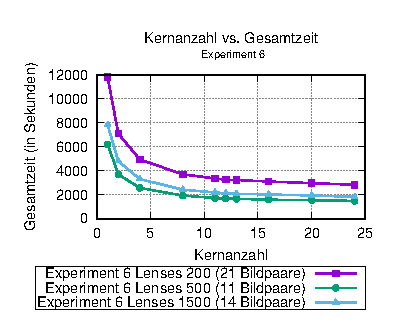
\includegraphics[width=\textwidth]{pdf/times_exp6}
			\caption[Experiment 6]{Experiment 6}
			\label{fig:times_exp6}
		\end{subfigure}
		\hfill
		\begin{subfigure}[b]{0.49\textwidth}
			\centering
			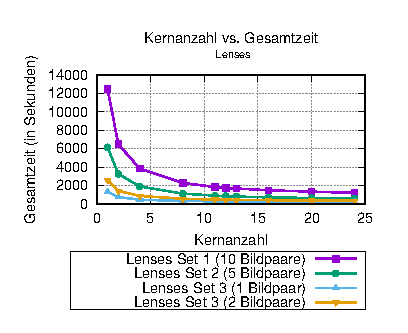
\includegraphics[width=\textwidth]{pdf/times_lenses}
			\caption[Lenses]{Lenses}
			\label{fig:times_lenses}
		\end{subfigure}
		\caption{Gesamtlaufzeiten}
		\label{fig:gesamtlaufzeiten}
	\end{figure}
\end{center}

Der Speedup des Programmes skaliert mit der Anzahl der Prozessorkerne nicht linear und flacht schnell ab. Der Speedup-Faktor für den \textit{Experiment 6} Datensätze übersteigt fünf nicht. Bei den \textit{Lenses}-Da\-ten\-sä\-tzen hingegen wird bei 24 Kernen ein Speedup von mehr als zehn erreicht. In den auf Abbildung \ref{fig:speedup} visualisierten Graphen ist eine starke Skalierung deutlich erkennbar. 

\begin{center}
	\begin{figure}
		\begin{subfigure}[b]{0.49\textwidth}
			\centering
			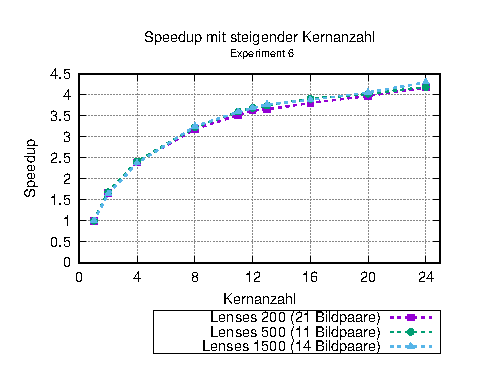
\includegraphics[width=\textwidth]{pdf/speedup_exp6}
			\caption[Experiment 6]{Experiment 6}
			\label{fig:speedup_exp6}
		\end{subfigure}
		\hfill
		\begin{subfigure}[b]{0.49\textwidth}
			\centering
			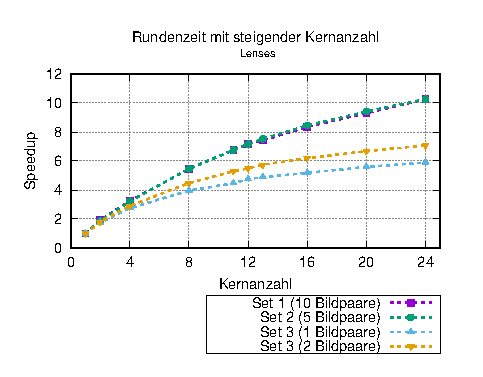
\includegraphics[width=\textwidth]{pdf/speedup_lenses}
			\caption[Lenses]{Lenses}
			\label{fig:speedup_lenses}
		\end{subfigure}
		\caption{Speedup}
		\label{fig:speedup}
	\end{figure}
\end{center}

Um Engpässe und besonders rechenaufwendige Funktionen zu identifizieren, wurde das Programm mit Zeitmessern versehen, die Ausführungszeiten und Aufrufanzahl protokolliert haben. Anschließend wurden es auf einem Rechenkern unter denselben Bedingungen, wie die anderen Konfigurationen, die Zeiten gemessen. Ein Überblick über das Gesamtprogramm mit seinen Subroutinen und deren Anteil an der Gesamtlaufzeit ist in Abbildung \ref{fig:perc_main} zu sehen.

\begin{center}
	\begin{figure}[htbp]
		\centering
		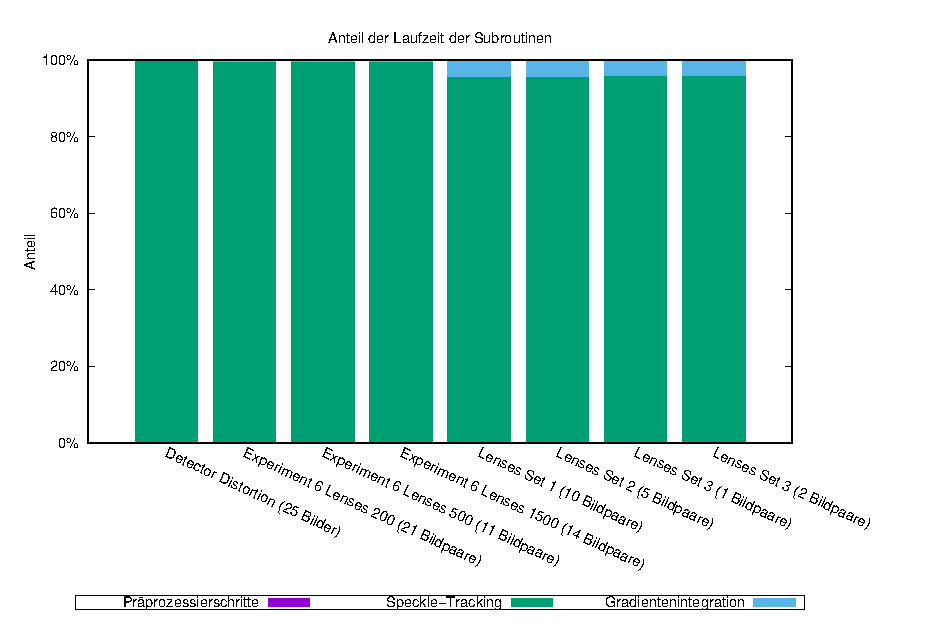
\includegraphics[width=0.7\textwidth]{pdf/main}
		\caption{Anteile der Laufzeiten}
		\label{fig:perc_main}
	\end{figure}
\end{center}

Hierbei ist eindeutig zu sehen, dass die meiste Zeit für das Speckle-Tracking benötigt wird. um weitere Informationen über die Laufzeiten der einzelnen Speckle-Tracking-Schritte zu gewinnen, wurde dieses ebenfalls mit Zeitmessern versehen. Die zeitliche Aufteilung dieser zeigt in Abbildung \ref{fig:perc_speckle}, dass hierbei der zweite Durchlauf am meisten Zeit benötigt. 

\begin{center}
	\begin{figure}[htbp]
		\centering
		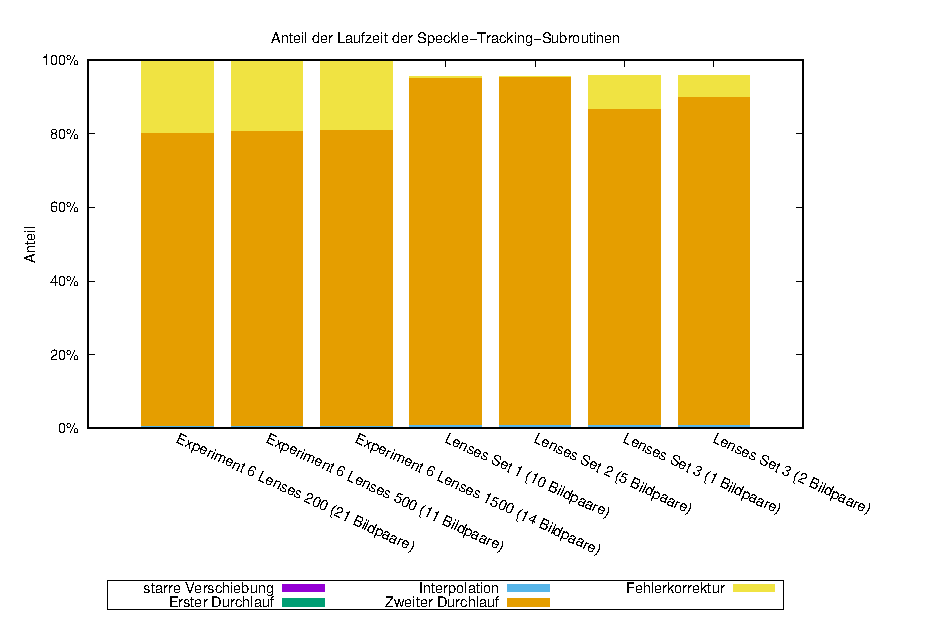
\includegraphics[width=0.7\textwidth]{pdf/speckle}
		\caption{Anteile der Laufzeiten des Speckle-Tracking-Algorithmus}
		\label{fig:perc_speckle}
	\end{figure}
\end{center}

Die kumulative Zeit der fünf rechenaufwendigsten Funktionen aller Konfigurationen, dargestellt in Abbildung \ref{fig:perc_slow}, liegt jeweils bei über 95\% der Gesamtzeit. 

\begin{center}
	\begin{figure}[htbp]
		\centering
		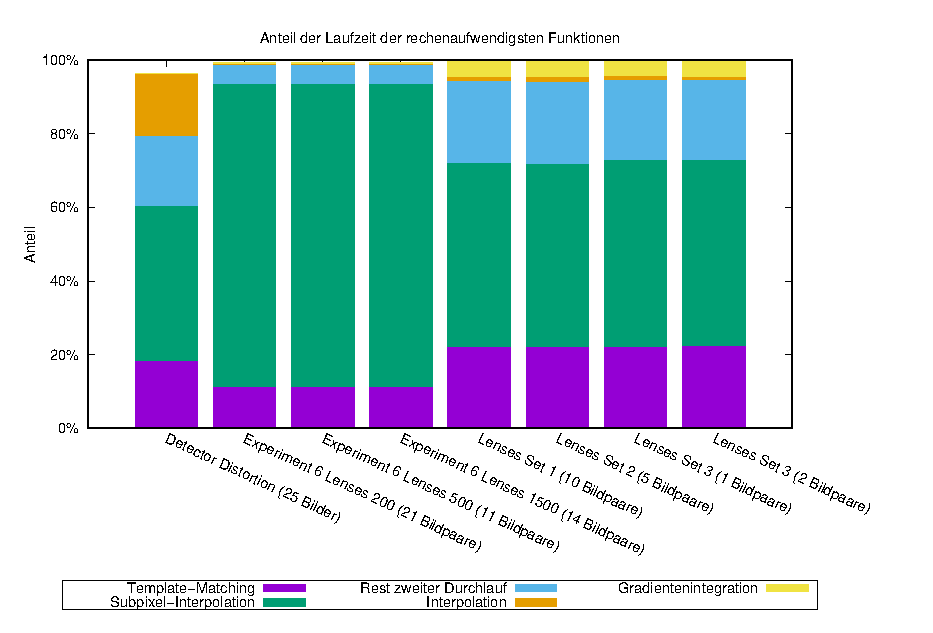
\includegraphics[width=0.7\textwidth]{pdf/slow}
		\caption{Anteile der Laufzeiten der langsamsten Funktionen}
		\label{fig:perc_slow}
	\end{figure}
\end{center}

\section{Grund der Performance-Engpässe}

Der Grund der langen Rechenzeiten des Template-Matchings und der Subpixel-Interpolation liegt in der hohen Anzahl der Aufrufe dieser begründet. Der zweite Durchlauf allein wird im \textit{Experiment 6 Lenses 200}-Datensatz über 5.3 Millionen mal aufgerufen. In jedem dieser Aufrufe wird das Template-Matching und die Subpixel-Interpolation jeweils ein mal genutzt. Hinzu kommt, dass, bis auf das Temp\-late-Match\-ing, der zweite Durchlauf nur geringen Gebrauch von bereits optimierten Bibliotheken wie numpy macht und somit der Pyhton-Overhead hinzukommt. 

Innerhalb des Speckle-Trackings ist der Aufruf des zweiten Durchlaufes mittels der joblib parallelisiert. Diese nutzt standardmäßig die multiprocessing-Bibliothek, welche für jeden Thread einen Fork der gesamten Python-Umgebung erstellen muss, was zu einem erheblichen Overhead führt\footnote{\url{https://pythonhosted.org/joblib/parallel.html}}.

Die hohe Rechenzeit der Gradienten-Integration ist im Aufruf dieser auf die Größe des Gesamtbildes begründet.

Insgesamt hat das Programm eine schlechte CPU-Auslastung von lediglich durchschnittlich 19,635\% \footnote{\url{https://github.com/ComputationalRadiationPhysics/Wavefront-Sensor/blob/f2fc5c2e5f8b4ef0e9b3ca3a4e770db67f230588/doc/cpu_util.md}}, wodurch häufig einige Kerne nicht oder nur wenig genutzt werden. 
	\chapter{Parallelisierung der kritischen Abschnitte}

Um der optimalen Leistung nah zu kommen wurde bei der Implementierung ein iterativer Ansatz gewählt. Hierzu wurden zuerst die Möglichkeiten der Parallelisierung und anschließend die, der Optimierung in Python betrachtet. 

\section{Parallelisierung}

\subsection{Parallelisierung der Verarbeitung einzelner Bildpaare mittels MPI}

Da die zu bearbeitenden Bildpaare voneinander unabhängig sind, lassen diese sich trivial parallelisieren. Der Vorteil dieses Ansatzes liegt besonders in seiner simplen Implementierung und erwarteten linearen Skalierung begründet. Dieser Ansatz bringt allerdings auch einige Nachteile mit sich: Viele \gls{MPI}-Implementierungen erlauben keine neuen \correctme{Threads Nachweiß einfügen} und es ist nur eine schwache Skalierung zu erwarten. Sofern kein Multithreading innerhalb von \gls{MPI} möglich ist, limitiert die Anzahl der Bildpaare die Parallelisierungsmöglichkeiten stark, weshalb hier aus Zeitgründen auf intensives Testen dieser Version verzichtet wird. 

\subsection{Parallelisierung innerhalb der Verarbeitung einzelner Bildpaare mittels MPI}

Eine sinnvolle Erweiterung zur oben beschriebenen Methode ist das Ersetzen der genutzten Multithreading-Bibliothek mittels MPI, sodass selbst die Berechnung eines einzelnen Bildpaares über Rechnergrenzen hinweg möglich ist. In diesem Zuge wurde auch die Fehlerkorrektur am Ende des Speckle-Trackings parallelisiert, indem die zu korrigierende Bildausschnitte auf mehrere Kerne verteilt wurden. Zusätzlich ermöglicht diese Implementierung den Einsatz eines Tracing-Programmes, wie SCORE-P\footnote{\url{http://www.vi-hps.org/projects/score-p/}}. Dies war aufgrund der unterliegenden multiprocessing-Bibliothek zuvor nicht möglich. Ein hoher Speedup wird insbesondere für wenige zu korrigierende Bildausschnitte nicht erwartet. 

Im konkreten werden die Bildpaare auch \gls{CPU}-Kern Gruppen verteilt. Einer dieser Kerne agiert hierbei als Hauptkern und ist dafür verantwortlich das Bildpaar zu verarbeiten, wobei dieser Aufgaben mittels eines \gls{MPI}-Kommunikators an die anderen Rechenkerne verteilen kann. Dies ist in der Abbildung \correctme{Abbildung einfügen} gezeigt. Die Schnittstelle wurde hierbei ähnlich zur joblib-Implementierung entworfen. Sollten mehr Bildpaare als Rechenkerne vorhanden sein, werde mehrere Bildpaare von eine Kern hintereinander verarbeitet. Die Programmierschnittstelle wurde so entworfen, dass die Verteilung der Bildpaare auf die Kernen und das Parallelisieren innerhalb dieser für den Programmierer transparent geschieht. \correctme{Implementierung verlinken}

\correctme{\textbf{Schemata einfügen}}

\section{Optimierung der Python-Engpässe}

\begin{correctmore}
	- Optimieren einzelner in Python implementierter Programmteile, die sich als besonders langsam herausgestellt haben
\end{correctmore}

\subsection{Nutzen von bereits optimierter Funktionen}

Einige Teile des Codes können durch bereits in Python oder einer optimierten Bibliothek enthaltenen Funktion ersetzt werden, womit der Interpretieraufwand erheblich reduziert wird. Dies gehört damit zu einer der grundlegenden Optimierungsmöglichkeiten. Zusätzlich dazu sind diese Funktionen meist bereits für optimale Leistung optimiert. In der Funktion \textit{nxcorr\_disp} lassen sich solche Code-Abschnitte finden. Die Code-Auflistung \correctme{Auflistung referenzieren} zeigt die Implementierung in reinem Python und die Auflistung \correctme{Auflistung referenzieren} zeigt die Nutzung von bereits optimierten Funktionen. 

\begin{lstlisting}
for i in range(1,lengthY-1):
	for j in range(1,lengthX-1):
		if (nxcorr[i, j] > maxValue):
			maxValue = nxcorr[i, j]
			maxI = i
			maxJ = j
\end{lstlisting}

\begin{lstlisting}
nxcorr_small = nxcorr[1:-1,1:-1]
(_, maxValue, _, (maxJ, maxI)) = cv2.minMaxLoc(nxcorr_small)
maxI += 1
maxJ += 1
\end{lstlisting}

Des weiteren befindet sich in der \textit{nxcorr\_disp}-Funktion die Berechnung des Signal-Rausch-Verhältnisses (gezeigt in Auflistung \correctme{Auflistung referenzieren}), was allerdings im weiteren Verlauf des Programmes nicht wieder verwendet wird. 

\begin{lstlisting}
avg = 0.0
count = 0
for i in range(lengthY):
	for j in range(lengthX):
		if ((i is not maxI) and (j is not maxJ)):
			avg = avg + abs(nxcorr[i,j])
			count = count + 1
avg = avg / float(count)
SNr = maxValue / avg
\end{lstlisting}

Nachdem diesen Änderungen befindet sich keine in Python implementierte Schleife mehr in der Funktion. Angesichts der hohen Aufrufzahl der \textit{nxcorr\_disp} und dem Entfernen großer Codeanteile ist ein hoher Beschleunigungsfaktor zu erwarten. \correctme{Implementierung verlinken}

\subsection{Kompilieren}

Eine weitere Möglichkeit der Minimierung des Python-Engpasses ist die Übersetzung des Codes in nativen Maschinencode. Die möglichen Ansätze hierbei reichen von der Übersetzung des gesamten Programmes über die Übersetzung einzelner Funktionen, die in Python dann als Modul geladen werden können, bis hin zur Nutzung eines just-in-time Compilers, welcher annotierte Funktionen bei dessen ersten Aufruf in nativen Maschinencode übersetzt. 

\subsubsection{Gesamtes Programm}

\begin{correctmore}
	- kompilieren des kompletten Projektes mit Cython
	- funktioniert, aber Ergebnisse bringen nicht gewünschten Speedup bzw. nur manchmal
	--> Ansatz verworfen
\end{correctmore}

\subsubsection{Einzelne Funktionen}

\correctme{ - kompilieren einzelne Funktion}

\paragraph{numba}

\correctme{ - just in time compiler}

\paragraph{Cython}

\begin{correctmore}
	- regulärer Compiler
	- weitere Optimierungsmöglichkeiten (z.B. mit C Typen)
\end{correctmore}
	\chapter{Performance-Messungen der parallelen Implementation}

Für die in diesem Kapitel durchgeführten Performance-Messungen wurde dasselbe Testsystem genutzt wie auch in Sektion \ref{sec:performance-messungen} beschrieben wurde. Die einzige Änderung hierbei ist, dass in vielen Benchmarks mehr als ein Knoten beansprucht wurde. Auch die Datensätze und die geladenen Module haben sich nicht geändert. Wie auch bei der Performance-Analyse, sind aus allen in diesem Kapitel angegeben Zeiten die \gls{IO}-Zeiten herausgerechnet worden. Ebenfalls wurde hier auch wieder nach vier Aufwärmiterationen für fünf Iterationen des Programmes die Zeit gemessen. 

\section{Evaluierung der Optimierungen}

\subsection{Parallelisierung}

Auf der Abbildung \ref{fig:mpi_speedup} ist für die auf dem GitHub-Branch \textit{mpi} verfügbare Version \cite{CBS18} deutlich ein Beschleunigungsfaktor von ca. zwei bis vier gegenüber der vorgegebenen Implementierung erkennbar. Anzumerken ist hierbei, dass als Referenz für den Speed-Up die Laufzeit der vorgegebenen Implementierung auf einem Kern genutzt wurde. Ebenfalls wird ersichtlich, dass diese Lösung nur mit der Anzahl der Eingabebildpaare skaliert, weshalb nur die \textit{Experiment 6 Lenses 200} und \textit{Lenses 500} mit 24 Kernen schneller ist als mit zwölf. Wie in Abbildung \ref{fig:mpi_times} zu sehen ist, liegen alle Laufzeiten dieser Version unter 1.000 Sekunden. Auch hier sind die Messpunkte wieder dick hervorgehoben und die Skala der Gesamtzeitgraphen ist logarithmisch eingeteilt. Ein Rechenknoten besitzt 24 Kerne, wodurch die Einteilung der X-Achse die Grenze der Rechenknoten verdeutlicht. 

\begin{center}
	\begin{figure}[h]
		\begin{subfigure}[b]{0.45\textwidth}
			\centering
			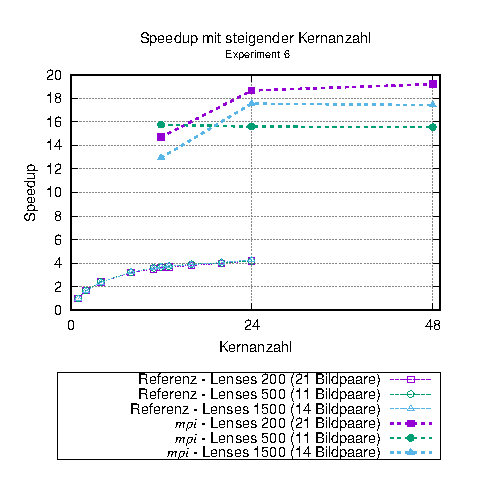
\includegraphics[width=\textwidth]{pdf/mpi_speedup_exp6}
			\caption{Experiment 6}
			\label{fig:mpi_speedup_exp6}
		\end{subfigure}
		\hfill
		\begin{subfigure}[b]{0.45\textwidth}
			\centering
			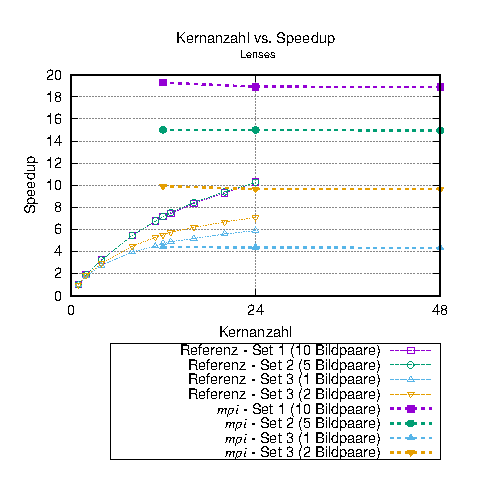
\includegraphics[width=\textwidth]{pdf/mpi_speedup_lenses}
			\caption{Lenses}
			\label{fig:mpi_speedup_lenses}
		\end{subfigure}
		\caption{Speed-Up der \textit{mpi} Implementierung gegenüber des von \citeauthor{Coj17} implementierten Python-Codes}
		\label{fig:mpi_speedup}
	\end{figure}
\end{center}

\begin{center}
	\begin{figure}[h]
		\begin{subfigure}[b]{0.45\textwidth}
			\centering
			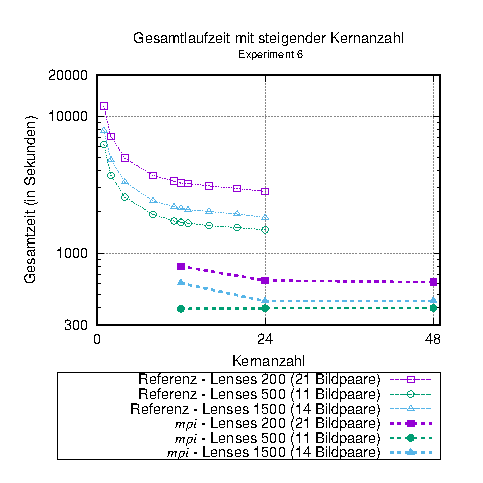
\includegraphics[width=\textwidth]{pdf/mpi_times_exp6}
			\caption{Experiment 6}
			\label{fig:mpi_times_exp6}
		\end{subfigure}
		\hfill
		\begin{subfigure}[b]{0.45\textwidth}
			\centering
			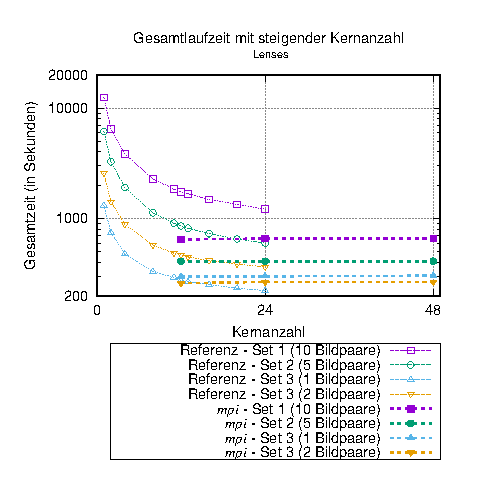
\includegraphics[width=\textwidth]{pdf/mpi_times_lenses}
			\caption{Lenses}
			\label{fig:mpi_times_lenses}
		\end{subfigure}
		\caption{Gesamtlaufzeit der \textit{mpi} Implementierung gegenüber des von \citeauthor{Coj17} implementierten Python-Codes}
		\label{fig:mpi_times}
	\end{figure}
\end{center}

Wie in Abbildung \ref{fig:mpi_advanced_speedup} zu sehen ist, schneidet die auf dem Branch \textit{mpi-advanced} verfügbare Version \cite{CBS18} für 24 Kerne schlechter ab als die \textit{mpi} Implementierung. Dies kann in der effizienteren Verteilung der Daten mittels der joblib-Bibliothek begründet liegen, da diese den in Linux effizient implementierten Fork-Befehl nutzt, wohingegen die \textit{mpi-advanced}-Implementierung die Daten direkt kopiert \cite{GVB+18}. Im Gegensatz zu der \textit{mpi}-Implementierung skaliert diese Version aber mit der Anzahl der verfügbaren \gls{CPU}-Kerne und nicht nur mit der Anzahl der Bildpaare. Anzumerken ist hier ebenfalls, dass die \textit{mpi}-Implementierung bei wenigen Kernen zwar schneller ist, aber deutlich mehr Arbeitsspeicher benötigt. Währenddessen die \textit{mpi-advanced}-Version unter Nutzung von 24 Kernen mit 64 \gls{GiB} auskommt, benötigt die \textit{mpi}-Version mehr als 128 \gls{GiB}.

Auch in der Abbildung \ref{fig:mpi_advanced_speedup} wurde wieder die auf einem Kern ausgeführte vorgegebene Implementierung als Referenz genutzt. 

\begin{center}
	\begin{figure}[h]
		\begin{subfigure}[b]{0.45\textwidth}
			\centering
			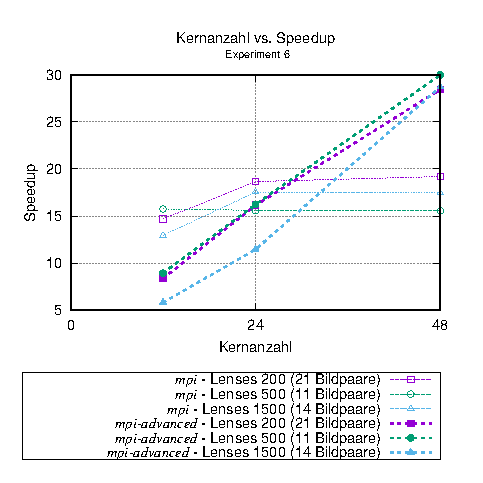
\includegraphics[width=\textwidth]{pdf/mpi_advanced_speedup_exp6}
			\caption{Experiment 6}
			\label{fig:mpi_advanced_speedup_exp6}
		\end{subfigure}
	\hfill
		\begin{subfigure}[b]{0.45\textwidth}
			\centering
			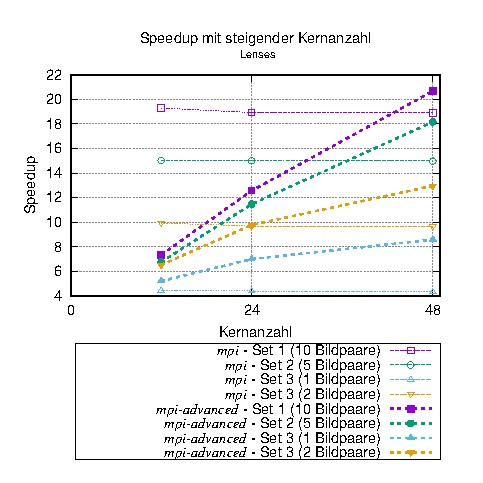
\includegraphics[width=\textwidth]{pdf/mpi_advanced_speedup_lenses}
			\caption{Lenses}
			\label{fig:mpi_advanced_speedup_lenses}
		\end{subfigure}
		\caption{Speed-Up der \textit{mpi-advanced} Implementierung gegenüber der \textit{mpi}-Version}
		\label{fig:mpi_advanced_speedup}
	\end{figure}
\end{center}

\begin{center}
	\begin{figure}[h]
		\begin{subfigure}[b]{0.45\textwidth}
			\centering
			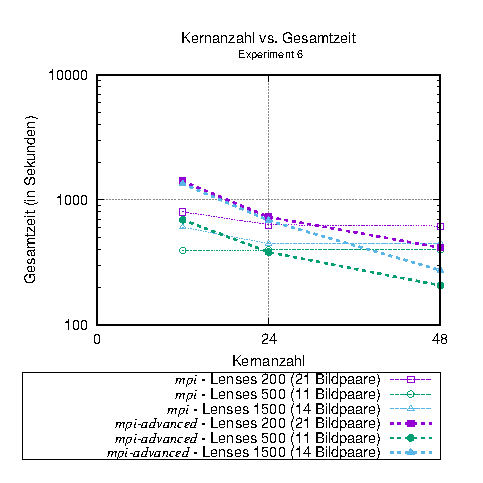
\includegraphics[width=\textwidth]{pdf/mpi_advanced_times_exp6}
			\caption{Experiment 6}
			\label{fig:mpi_advanced_times_exp6}
		\end{subfigure}
		\hfill
		\begin{subfigure}[b]{0.45\textwidth}
			\centering
			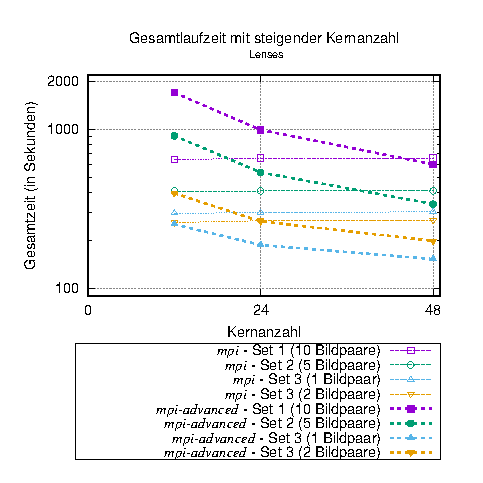
\includegraphics[width=\textwidth]{pdf/mpi_advanced_times_lenses}
			\caption{Lenses}
			\label{fig:mpi_advanced_times_lenses}
		\end{subfigure}
		\caption{Gesamtlaufzeit der \textit{advanced-mpi} Implementierung gegenüber des von Cojocaru implementierten Python-Codes}
		\label{fig:mpi_advanced_times}
	\end{figure}
\end{center}

\subsection{Optimierung von Python-Engpässen}

\subsubsection{Nutzen bereits optimierter Funktionen}

Wie in Abbildung \ref{fig:speedups_intrinsics} zu sehen ist, wurde mittels der Nutzung von bereits optimierten Funktionen ein Beschleunigungsfaktor von ca. vier für die \textit{Experiment 6}-Datensätze und ein Faktor zwischen 1,2 und 1,5 für die \textit{Lenses}-Datensätze erreicht. Der Speed-Up bei diesen Datensätzen war nicht so hoch, da diese weniger Bildpaare beinhalten und die Rechenzeit pro Bildpaar deutlich kleiner war, wodurch der Overhead durch das Senden der Daten einen größeren Einfluss auf die Gesamtlaufzeit hat. Die geringere Rechenzeit pro Bildpaar kommt durch die deutlich kleinere \gls{ROI}, eine kleinere \glsfirst{corrsize} \glssymbol{corrsize} und weniger zu korrigierenden Teilbilder zustande. Zusätzlich dazu entfällt die Notwendigkeit der Interpolation zwischen zwei verschiedenen Pixelgrößen, da hierfür nur ein Sensor im Einsatz war.

\begin{center}
	\begin{figure}[h]
		\begin{subfigure}[b]{0.54\textwidth}
			\centering
			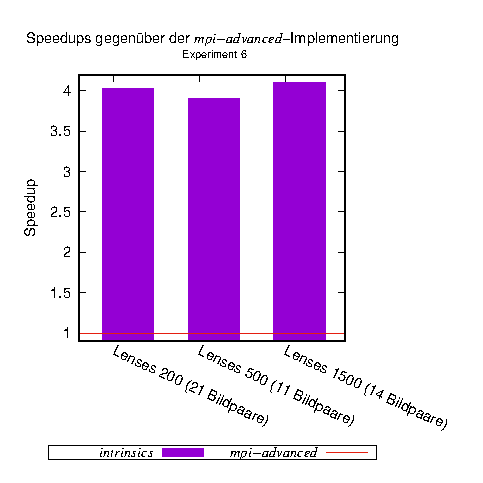
\includegraphics[width=\textwidth]{pdf/speedups_intrinsics_exp6}
			\caption{Experiment 6}
			\label{fig:speedups_intrinsics_exp6}
		\end{subfigure}
		\hspace{-0.9cm}
		\begin{subfigure}[b]{0.54\textwidth}
			\centering
			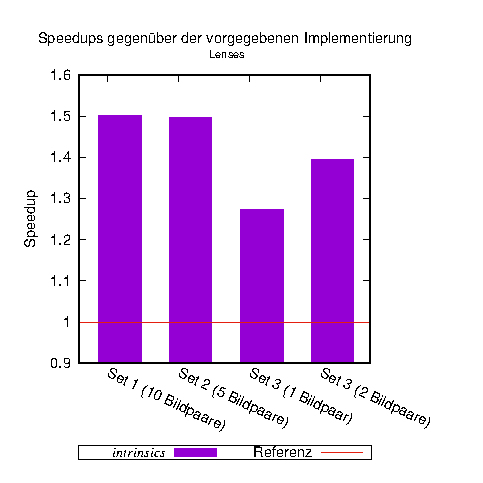
\includegraphics[width=\textwidth]{pdf/speedups_intrinsics_lenses}
			\caption{Lenses}
			\label{fig:speedups_intrinsics_lenses}
		\end{subfigure}
		\caption{Speed-Up der \textit{intrinsics} Implementierungen gegenüber der \textit{mpi-advanced}-Implementierung mit zwölf Kernen}
		\label{fig:speedups_intrinsics}
	\end{figure}
\end{center}

\begin{center}
	\begin{figure}[h]
		\begin{subfigure}[b]{0.54\textwidth}
			\centering
			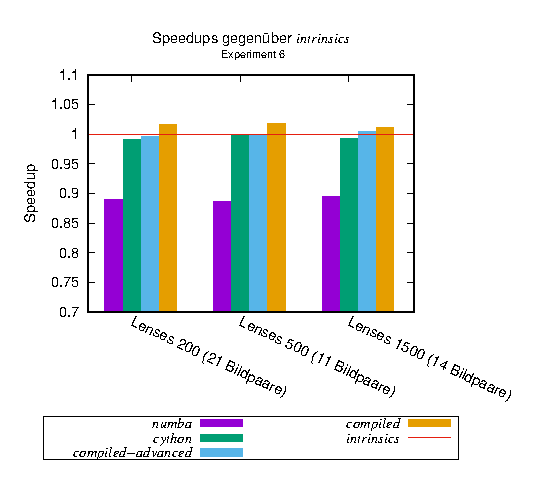
\includegraphics[width=\textwidth]{pdf/speedups_exp6}
			\caption{Experiment 6}
			\label{fig:speedups_exp6}
		\end{subfigure}
		\hspace{-0.9cm}
		\begin{subfigure}[b]{0.54\textwidth}
			\centering
			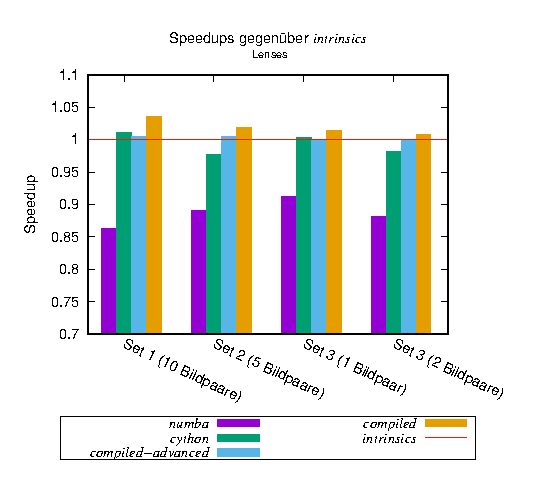
\includegraphics[width=\textwidth]{pdf/speedups_lenses}
			\caption{Lenses}
			\label{fig:speedups_lenses}
		\end{subfigure}
		\caption{Speed-Ups der einzelnen Implementierungen gegenüber der \textit{intrinsics} Implementierung mit zwölf Kernen}
		\label{fig:speedups}
	\end{figure}
\end{center}

\subsubsection{Kompilieren}

Die Abbildung \ref{fig:speedups} zeigt den Beschleunigungsfaktor der verschiedenen übersetzten Versionen gegenüber der Implementierung, welche bereits optimierte Funktionen nutzt. Hierbei ist deutlich ersichtlich, dass die Übersetzung des gesamten Programmes, welche auf dem \textit{compiled}-Branch verfügbar ist, immer schneller als die \textit{intrinsics}-Implementierung läuft. Der Grund für die höhere Leistung der \textit{compiled}-Implementierung ist hierbei nicht bekannt. Die \textit{numba}-Version hingegen schnitt immer deutlich schlechter als die anderen Versionen ab. Die Laufzeiten der \textit{cython}- und der \textit{compiled-advanced}-Versionen liegen nahe beieinander und bieten keinen Geschwindigkeitszuwachs gegenüber der \textit{intrinsics}-Implementierung. 

Die bereits gute Performance der \textit{intrinsics}-Implementierung liegt in der intensiven Nutzung optimierter Funktionen begründet, welche von einer Übersetzung der Python-Codes unberührt bleiben. Die Performance der \textit{numba}-Implementierung ist deutlich schlechter, da beim Aufruf einer \gls{JIT}-kompilierten Funktion diese erst in einer Liste aus übersetzten Funktionen gesucht werden muss, bevor diese aufgerufen werden kann \cite{PKA17}. Dieser Effekt wird dadurch verstärkt, dass die übersetzten Funktionen eine geringe Laufzeit haben, aber dafür sehr oft aufgerufen werden. Der zweite Durchlauf allein, und damit auch die \texttt{nxcorr\_disp()}-Funktion, wird im \textit{Experiment 6 Lenses 200}-Datensatz über 5.3 Millionen mal aufgerufen. 

\section{Skalierung}

Auf der Abbildung \ref{fig:best_speedup_standalone} ist eine lineare Skalierung gut erkennbar, bis die Anzahl der \gls{CPU}-Kerne die Anzahl der Bildpaare übersteigt. Anschließend stagniert der Beschleunigungsfaktor, da einige Bildpaare zwar mit mehr Kernen schneller bearbeitet werden können, aber das Programm auf die Fertigstellung der restlichen Bildpaare warten muss, die nur einen Kern zur Verfügung haben. Ein ähnliches Laufzeitverhalten lässt sich jedes Mal beobachten, wenn die Kernanzahl ein Vielfaches der Bildpaaranzahl erreicht. Da die Verarbeitung eines einzelnen Bildpaares nicht komplett parallelisiert werden kann, flacht laut Amdahl's Gesetz der Graph mit steigender Kernanzahl ab \cite{Amd67}. Die Gesamtlaufzeiten im Bezug auf die vorgegebene Implementierung ist in Abbildung \ref{fig:best_times} zu sehen. 

\begin{center}
	\begin{figure}[h]
		\begin{subfigure}[b]{0.45\textwidth}
			\centering
			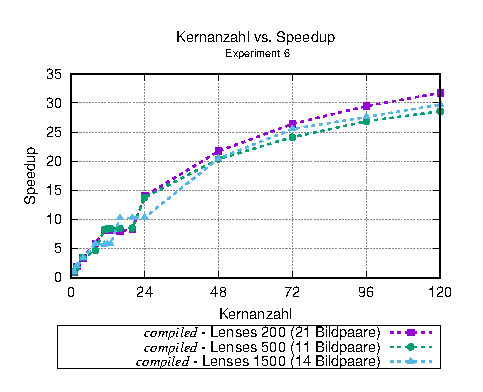
\includegraphics[width=\textwidth]{pdf/best_speedup_exp6_standalone}
			\caption{Experiment 6}
			\label{fig:best_speedup_exp6_standalone}
		\end{subfigure}
		\hfill
		\begin{subfigure}[b]{0.45\textwidth}
			\centering
			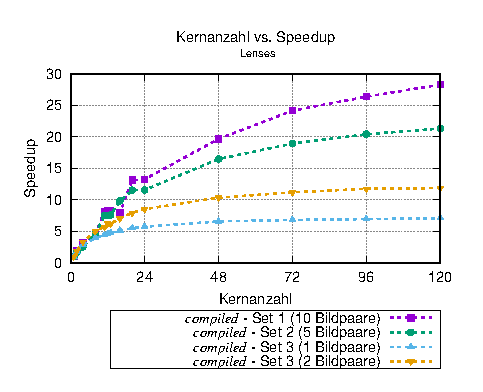
\includegraphics[width=\textwidth]{pdf/best_speedup_lenses_standalone}
			\caption{Lenses}
			\label{fig:best_speedup_lenses_standalone}
		\end{subfigure}
		\caption{Speed-Up der \textit{compiled} Implementierung}
		\label{fig:best_speedup_standalone}
	\end{figure}
\end{center}

\begin{center}
	\begin{figure}[h]
		\begin{subfigure}[b]{0.45\textwidth}
			\centering
			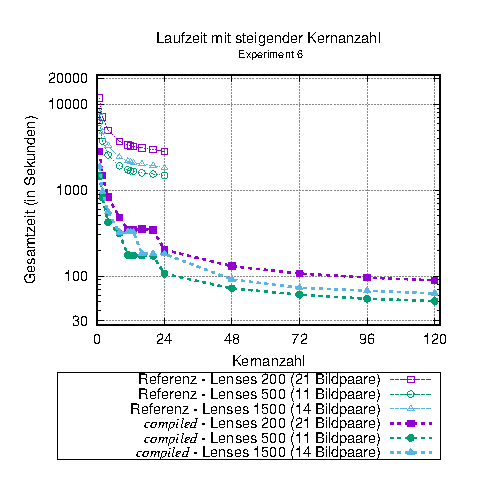
\includegraphics[width=\textwidth]{pdf/best_times_exp6}
			\caption{Experiment 6}
			\label{fig:best_times_exp6}
		\end{subfigure}
		\hfill
		\begin{subfigure}[b]{0.45\textwidth}
			\centering
			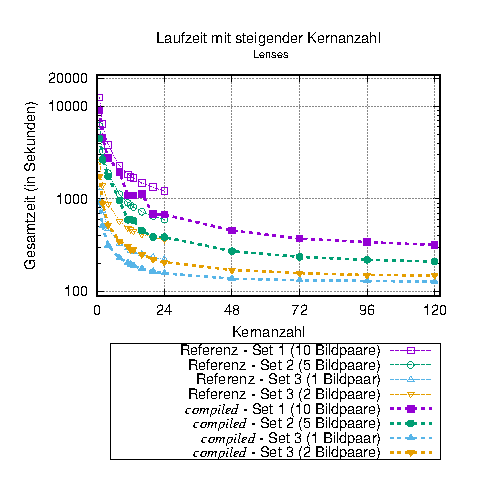
\includegraphics[width=\textwidth]{pdf/best_times_lenses}
			\caption{Lenses}
			\label{fig:best_times_lenses}
		\end{subfigure}
		\caption{Gesamtlaufzeit der \textit{compiled} Implementierung gegenüber des vorgegebenen Python-Codes}
		\label{fig:best_times}
	\end{figure}
\end{center}

Der Speed-Up-Graph in Abbildung \ref{fig:best_speedup_standalone} weist eine starke Skalierung auf, jedoch skaliert das Laufzeitverhalten schwach besser. Solang mehr Bildpaare als \gls{CPU}-Kerne an der Berechnung beteiligt sind, skaliert das Programm nahezu linear. Das Effizienzoptimum wird somit erreicht, wenn die Anzahl der \gls{CPU}-Kerne gleich der Anzahl der Bildpaare ist, da an diesem Punkt jeder Kern mit einem Bildpaar komplett ausgelastet ist und keine Zeit zum weiteren Verteilen der Daten aufgebracht werden muss. 

Eine Sättigung tritt bei allen Datensätzen ein, sobald mehr als 20 \gls{CPU}-Kerne pro Bildpaar eingesetzt werden. An diesem Punkt wird die meiste Rechenzeit in nicht parallelisierten Abschnitten des Speckle-Trackings und in der Gradientenintegration verbracht.
	\chapter{Auswertung}

\section{Wertung des Ergebnisses}

Die Abbildung \ref{fig:best_speedup} zeigt einen deutlich erhöhten Speedup gegenüber der vorgegebenen Python-Implementierung. Für die \textit{Experiment 6}-Datensätze erreicht dieser einen Speedup von über 130 und für die \textit{Lenses}-Datensätze liegt der maximale Beschleunigungsfaktor bei bis zu 40 für den \textit{Set 1}-Datensatz. Bei der Wahl größerer Datensätze sind aufgrund mangelnder Parallelisierbarkeit der Bildpaare größere Beschleunigungsfaktoren zu erwarten.

\begin{center}
	\begin{figure}[htbp]
		\begin{subfigure}[b]{0.45\textwidth}
			\centering
			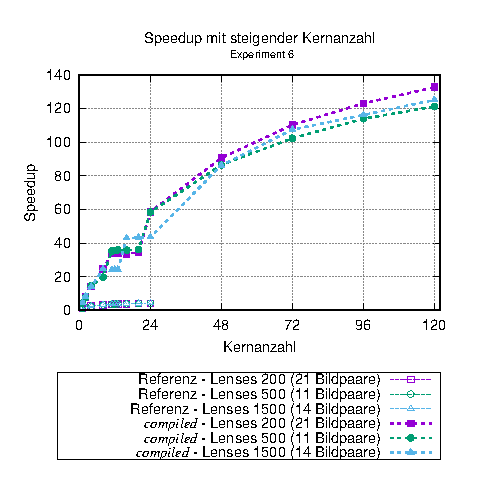
\includegraphics[width=\textwidth]{pdf/best_speedup_exp6}
			\caption{Experiment 6}
			\label{fig:best_speedup_exp6}
		\end{subfigure}
		\hfill
		\begin{subfigure}[b]{0.45\textwidth}
			\centering
			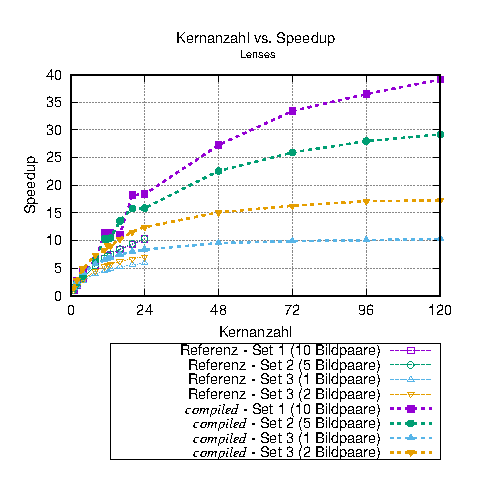
\includegraphics[width=\textwidth]{pdf/best_speedup_lenses}
			\caption{Lenses}
			\label{fig:best_speedup_lenses}
		\end{subfigure}
		\caption{Speedup der \textit{compiled} Implementierung gegenüber des von Cojocaru implementierten Python-Codes}
		\label{fig:best_speedup}
	\end{figure}
\end{center}

Trotz dessen, dass mit 120 \gls{CPU}-Kernen bereits ein Speedup von über 130 erreicht wurde, müsste die Anzahl der Bildpaare und der Kerne bei weitem höher sein, um die Echtzeitfähigkeit des Programmes sicher zu stellen. Dies ist in Größenordnungen von 2400 Bildpaaren und 2400 \gls{CPU}-Kernen zu erwarten, was bereits 100 Taurus-Knoten wären. 

\section{Verbesserungsmöglichkeiten}

Im Verlauf der Implementierung wurden viele der trivialsten Optimierungsmöglichkeiten implementiert. Während der letzten Iterationen der Implementierungen wurde allerdings auch weiteres Potential sichtbar. Beispielsweise ließe sich die Knoten interne Kommunikation mit Intrakommunikatoren oder geteiltem Speicher optimieren um den Kopieraufwand der Daten zu senken. 

Obwohl in dieser Arbeit bereits viele Optimierungen implementiert wurden und ein hoher Speedup erreicht wurde, gibt es immer noch weiteres Potential. Die Verwendung der FFTW\footnote{\url{http://www.fftw.org/}}-Bibliothek ist eine davon. Mithilfe dieser ist es möglich, die Gradientenintegration zu beschleunigen indem beim Start des Programmes sogenannte \textit{Wisdoms} erstellt werden, welche die Transformation eines Bildes in den Frequenzraum erheblich beschleunigen könnte. 

Des Weiteren ist es möglich für die am häufigsten aufgerufenen Funktionen Datenblöcke zu bilden und diese zu verarbeiten, sodass der Overhead der Funktionsaufrufe sinkt. Dies bildet ebenfalls eine gute Grundlage um diese Datenblockverarbeitung mittels numpy, numexpr oder numba weiter zu beschleunigen. Insbesondere kann hierbei auch die CUDA\footnote{\url{https://developer.nvidia.com/cuda-zone}} und OpenCL\footnote{\url{https://www.khronos.org/opencl}} Schnittstelle von numba genutzt werden, um Berechnungen mittels \glspl{GPGPU} auszulagern. 

Eine weitere Verbesserungsmöglichkeit liegt in einer Verbesserung des Belastungsausgleiches. Hierbei bestünde die Möglichkeit die Bildpaare in Packete zusammenzufassen und diese hintereinander auszuführen, sodass ein durchgängiger Betrieb möglich wäre. 

Auch Optimierungen am Algorithmus sind noch denkbar. Da aus dem Ergebnis des Template-Matchings nur die Position und der Wert des Maximums benötigt werden, ließe sich Bild und Template mit durch Skalierung verminderter Auflösung matchen. Hierbei entstandene Ungenauigkeiten können behoben werden, indem in der Region des Maximums ein genaueres Match durchgeführt wird. Da das Match mit reduzierter Auflösung eine Heuristik über die Maximal mögliche Übereinstimmung ist, kann anschließend in diesem der zweit höchste Wert betrachtet werden. Ist dieser größer als das Ergebnis des genauen Matches, besteht die Möglichkeit, dass dieses falsch ist und es kann auf den in der OpenCV-Bibliothek implementierten Template-Matching-Algorithmus zurückgreifen. Ist die Auflösung des Templates und des Bildes jedoch nicht durch ein und denselben Skalierungsfaktor teilbar, so kann die Skalierung auf eine niedrigere Auflösung bereits erhebliche Zeit in Anspruch nehmen. Hierzu ähnliche Optimierungsmöglichkeiten wurden bereits von Elena-Ruxandra Cojocaru implementiert (siehe \ref{sec:speckle-tracking}). 

Zu guter Letzt besteht auch noch die Möglichkeit der Optimierung des Kalibrierungsteiles des Programmes. 
	\appendix
	\printbibliography

\end{document}